%% MethodsX methods article -- Elsevier elsarticle template
%% Structure follows the official "MethodsX methods article template
%% Version 7 (September 2024)". Section headings match the template and must
%% not be changed. All sections are mandatory unless marked OPTIONAL.
%%
%% Compile with pdfLaTeX (run twice to resolve \cite references).
%% Overleaf: New Project -> Upload Project -> Compiler = pdfLaTeX.
%%
%% LAYOUT: 'final,3p' = journal single-column look (for reading / advisor
%%   review). When you SUBMIT, change 'final' to 'review' for the
%%   double-spaced, line-numbered manuscript format Elsevier expects.
%%
%% TODO before submitting:
%%   - fill every [bracketed] placeholder (affiliations, ethics,
%%     funding, CRediT roles);
%%   - prepare the Graphical abstract as a SEPARATE image file;
%%   - delete this comment header.
%%
%% DO NOT SUBMIT UNTIL THESE TWO ARE RESOLVED (2026-08-11):
%%
%%   1. The 92.7 % scanning precision (abstract, and the "Reliability of the
%%      detections" paragraph) is NOT a valid estimate of precision above 0.95.
%%      The 55 clips came from export_detection_clips.py --reliability, which
%%      samples the confidence axis evenly rather than the detections: 41 of the
%%      55 were drawn from a pool of 73 detections (56 % inclusion) and 14 stand
%%      for the remaining 695 (2.0 %), a 28:1 ratio, then averaged unweighted.
%%      The Wilson interval assumes equal-probability sampling and is invalid for
%%      the same reason. Worse, the verdicts were never written down: all 185
%%      rows of IPA20ST_day_sheet.csv and IPA4ST_day_sheet.csv have an empty
%%      verdict column, so 51/55 cannot be reproduced from any file.
%%      REPLACEMENT IN PROGRESS: an equal-probability sample of 150 of the 768
%%      detections at >= 0.95 (seed 20260811, design in
%%      data/outputs/precision_resample/DESIGN.txt) is with the species expert.
%%      Report that result and its Wilson interval; state the sampling design.
%%
%%   2. The "117 of the 124 dawn candidates have more than 95 % of their energy
%%      above 1.5 kHz and cannot be a low-frequency roar" sentence is falsified
%%      by our own material: the confirmed field roar
%%      0.906_2_S1141_44100H_GRNP764_20211215_170000 has a low-frequency ratio
%%      of 0.0200, i.e. 98.0 % of its in-band energy above 1.5 kHz. The screen
%%      actually cut at 0.40, not at 95 %, and 56 of the 117 discarded windows
%%      sit at or above the lowest confirmed roar's ratio -- none of them heard.
%%      All 117 are with the species expert now. The count of screened-out
%%      windows cannot be reported as evidence of absence until they are.

\documentclass[final,3p,times]{elsarticle}

\usepackage{lineno,hyperref}
\usepackage{tabularx}
\usepackage{booktabs}
\usepackage{amssymb}
\usepackage[final]{graphicx}
\usepackage{float}
\usepackage[utf8]{inputenc}
\usepackage[T1]{fontenc}
\modulolinenumbers[5]

\journal{MethodsX}

\begin{document}

%% =====================================================================
%% ARTICLE INFORMATION
%% Title (max. 20 words), authors (mark corresponding with *), full
%% affiliations, corresponding e-mail (+ X handle), keywords (>= 3).
%% =====================================================================
\begin{frontmatter}

\title{Transfer-learning detection of primate vocalizations in
tropical-forest recordings with automatic false-positive cleanup}

\author[a]{Moshi Fu\corref{cor1}}
\ead{mfu39@wisc.edu}
\cortext[cor1]{Corresponding author.}

\author[a]{[Co-author Name]}

\affiliation[a]{organization={Department of Statistics, University of Wisconsin--Madison},
            addressline={150 Langdon Street},
            city={Madison},
            postcode={53703},
            state={WI},
            country={USA}}

\affiliation[b]{organization={[Second institution, full address]},
            country={[Country]}}

%% ABSTRACT -- max. 200 words, ending with 1-3 bullet points that
%% outline the method (no technical steps).
\begin{abstract}
%% TODO(Santi): review/expand the conservation-significance framing below.
Passive acoustic monitoring is a key tool for tracking vocal animals and
informing their conservation \textbf{[Santi --- please review / expand this
conservation-significance framing]}, but it produces thousands of hours of
audio that cannot be annotated by hand. The obstacle is precision: a classifier
trained on curated clips also fires on untrained forest sounds, so every
detection must be checked by ear. We target \textit{Cercopithecus nictitans}
and \textit{Colobus guereza} in Ivindo National Park, Gabon; only
\textit{C.\ nictitans} was
confirmed in the field, and the \textit{C.\ guereza} branch is reported as a
negative result. Mel-spectrograms are classified by a VGG19 transfer-learning
model with a frequency-position-aware CRNN head. Validated by a 16-fold
leave-one-station-out sweep over 6\,189 manually reviewed field detections,
retraining on human verdicts rather than filter guesses raises precision from
0.72 to 0.97 at a threshold fitted on the other stations, removing 94\,\% of
false positives while keeping 91\,\% of calls --- though recall is an outcome
rather than a constraint here and falls to 77\,\% at the worst station. The
fitted threshold varies widely
across held-out stations, so the fitting procedure transfers but its value does
not. Run as a scanner over raw audio rather than as a re-ranker, and checked by
ear, the retrained model returned 51 genuine calls in 55 confidence-stratified
detections above 0.95 at two stations --- \textbf{[a design-weighted precision
for that band, from an equal-probability sample of 150, is with the species
expert and replaces this sentence]}. A cleanup measured
against that same review
proves most useful not as a filter but as a way to organise listening: counting
a run of detections as one decision cuts the review to between an eighth and a
quarter of the clips while discarding nothing, and ordering what remains
recovers 90\% of the recoverable calls from half.

\begin{itemize}
\item A VGG19 transfer-learning model with a frequency-position-aware CRNN
head, hardened against forest-noise false positives.
\item A cleanup that groups and orders detections for review instead of
discarding them, measured against a review of every field detection.
\item A complete, reusable pipeline that recycles confirmed errors into
retraining and re-targets to new species by swapping in reference clips.
\end{itemize}
\end{abstract}

%% KEYWORDS -- minimum three, separated by \sep.
\begin{keyword}
Bioacoustics \sep Passive acoustic monitoring \sep Transfer learning \sep
Convolutional recurrent neural network \sep False-positive filtering \sep
\textit{Cercopithecus nictitans} \sep \textit{Colobus guereza}
\end{keyword}

\end{frontmatter}

%% =====================================================================
\section*{Related research article}
None.

%% =====================================================================
\section*{Graphical abstract}
Provided as a separate image file, per the MethodsX submission requirements.

%% =====================================================================
\section*{Specifications table}

\noindent
\renewcommand{\arraystretch}{1.3}
\begin{tabularx}{\linewidth}{@{}lX@{}}
\toprule
Subject area & Agricultural and Biological Sciences \\
More specific subject area & Bioacoustics; passive acoustic monitoring;
deep learning; conservation biology \\
Name of your method & CRNN Primate-Call Detector \\
Name and reference of original method & Transfer learning with the VGG19
architecture (Simonyan \& Zisserman, 2015) \cite{simonyan2015}; frequency-position
encoding adapted from CoordConv (Liu et al., 2018) \cite{liu2018}; spectrogram
data augmentation adapted from a rainforest-CNN pipeline (Sun et al., 2022)
\cite{sun2022}; out-of-distribution detection via the Mahalanobis distance
(Lee et al., 2018) \cite{lee2018}; audio event tagging with YAMNet trained on
AudioSet (Gemmeke et al., 2017; Hershey et al., 2017) \cite{gemmeke2017,hershey2017} \\
Resource availability & Code:
\url{https://github.com/mo119m/primates-sound-detection}, including
ready-to-run Jupyter notebooks and a step-by-step \texttt{SETUP.md}, with
pinned dependencies for an exactly reproducible environment. Python 3,
TensorFlow 2, librosa, scikit-learn, OpenCV, soundfile; the YAMNet filter
additionally needs tensorflow-hub. The trained model weights and curated
reference clips are available from the corresponding author on reasonable
request. \\
\bottomrule
\end{tabularx}

%% =====================================================================
%% BACKGROUND -- motivation and context. Max. 500 words.
%% =====================================================================
\section*{Background}

Passive acoustic monitoring is now a standard tool for surveying vocal animals
across large areas and long time spans, but it generates volumes of audio that
cannot realistically be reviewed by ear \cite{cauzinille2024}. Deep convolutional
networks applied to spectrogram ``images'' have become the dominant approach
for automatically detecting species-specific calls, and transfer learning from
large image or audio corpora lets such detectors be trained from comparatively
few annotated examples \cite{sun2022}. These approaches work well
on curated, isolated reference clips.

The difficulty in practice is precision rather than recall. A model trained on
curated clips of a target call will reliably fire on those calls, but when it
is run over continuous field recordings it also fires on the many non-target
sounds that dominate a rainforest soundscape (insects, birds, wind, rain,
and the calls of non-target animals), none of which are well represented in
the original training set. The result is a detector with a high false-positive
rate, and verifying every detection by hand reintroduces exactly the
manual-listening bottleneck that automation was meant to remove.

This method addresses that problem for two primate species recorded in Ivindo
National Park, Gabon: \textit{Cercopithecus nictitans},
whose repertoire includes acoustically distinct ``hack'', ``kek'', and
``pyow'' call types \textbf{[cite the putty-nosed call-type source, confirm
the reference with the species expert]}, and \textit{Colobus guereza}.

Two colobines have range records covering this area. \textit{C.\ guereza} ssp.
\textit{occidentalis} is listed as occurring in Ivindo National Park, and the
Ogooué River south of the park marks the lower elevation limit of its
range~\cite{iucnguereza2025}; \textit{C.\ satanas} ssp. \textit{anthracinus},
the Gabon black colobus, also has range covering
Gabon~\cite{iucnsatanas2020}. The two vocalise very differently, so a detector
built on reference material from one is not evidence about the other, and the
result reported here concerns \textit{C.\ guereza} alone. The area is
otherwise poorly surveyed: most published work on \textit{C.\ satanas} in
Gabon comes from Lopé National Park rather than from Ivindo, and no systematic
biodiversity inventory covers these stations. That gap is the reason a null
acoustic result here carries information rather than merely failing to confirm
what was already known.
%% TODO(Santi): expand the background below.
\textbf{[Santi --- please add more background here, e.g.\ the conservation /
IUCN status of the two species and why acoustic monitoring matters for their
conservation.]}
Rather
than only training a classifier, we wrap it in (i) a detection stage with
domain-appropriate post-processing, (ii) an automatic cleanup that flags
likely false positives using signals independent of the detector itself, and
(iii) an iterative hard-negative mining loop that recycles
confirmed false positives into the background class and retrains. The
motivation is to obtain trustworthy detections from long recordings while
keeping the amount of manual listening close to zero, and to do so with a
workflow that other researchers can re-run on their own species by supplying
new reference clips and editing a single configuration file.

%% =====================================================================
%% METHOD DETAILS -- enough detail to reproduce the method. No word limit.
%% =====================================================================
\section*{Method details}

The pipeline has five stages (preprocessing, training, detection, automatic
cleanup, and iterative retraining), augmented by three targeted
false-positive controls for \textit{Colobus}: a frequency-position-aware
classifier head that encodes where in frequency a call sits, a
dedicated hard-negative ``confuser'' class learned during training, and a
calibrated low-frequency energy gate applied at detection time. All paths,
species definitions, and hyperparameters live in a single configuration file so
the workflow can be re-targeted to new species or sites without touching the
code.

\subsection*{Study area, recordings, and reference clips}

Field recordings are continuous WAV files collected at fixed acoustic stations
(denoted IPA1ST, IPA2ST, \dots; one subfolder per recording date) in
rainforest in Ivindo National Park, Gabon, near Makokou.

The model is trained on short reference clips organized into four classes
(Table~\ref{tab:traindata}):
\begin{itemize}
\item \textbf{Cernic}: all putty-nosed monkey call types (putty-nose, hack,
kek, pyow) pooled into a single class. Five source folders (one per call type
plus a folder of recovered field calls) are mapped to
the single ``Cernic'' label, so that
merging happens at training time and the model directly outputs a unified
putty-nosed decision;
\item \textbf{Colobus\_guereza}: \textit{Colobus guereza} reference calls;
\item \textbf{Colobus\_confuser}: a dedicated hard-negative class containing
the forest sounds that earlier model versions repeatedly mis-fired as
\textit{Colobus}, mined from field detections across the development stations
and human-reviewed so that no genuine target call is included.
Giving the confuser its own softmax output forces the model to learn the
\textit{Colobus}-vs-confuser boundary explicitly instead of diluting these few
hundred hard negatives inside the much larger generic Background class; at
detection time the class is folded back into the background group (see
the detection-grouping and hard-negative-mining stages below) so it never
produces a detection;
\item \textbf{Background}: a pooled negative class assembled from ambient
forest noise, calls of non-target animals present at the site (e.g.\
\textit{Cercocebus torquatus}, \textit{Pan troglodytes}), and previously
misclassified clips recycled through the hard-negative mining loop.
\end{itemize}

\begin{table}[H]
\centering
\caption{Training-data composition: human-verified reference clips per class,
before augmentation.}
\label{tab:traindata}
\begin{tabularx}{\linewidth}{lrX}
\toprule
Class & Clips & Composition \\
\midrule
Cernic            & 3{,}002      & 2{,}535 reviewed field detections, 397
                                   reference calls (putty-nose, hack, kek,
                                   pyow), 70 recycled false positives \\
Colobus\_guereza  & 665          & roar pulses segmented from
                                   \textit{C.\ guereza} reference recordings \\
C\_pogonias       & 150          & \textit{C.\ pogonias} clips from reference
                                   recordings \\
Colobus\_confuser & 907          & 654 curated hard-negatives, 253
                                   field false positives, all human-reviewed \\
Background        & 25{,}891     & 16{,}826 BirdNET bird detections from the
                                   wider Gabon recording programme (\S\,below),
                                   3{,}654 reviewed non-calls, 3{,}460
                                   recycled false positives, 1{,}951 reference
                                   recordings of non-target species \\
\midrule
\textbf{Total}    & 30{,}615     & \\
\bottomrule
\end{tabularx}
\end{table}

\noindent These are raw clip counts, before augmentation
(\S\,Data augmentation). Per-class validation totals are deliberately not
reported; see \S\,Model training for why a validation accuracy on this pool was
withdrawn, and Table~\ref{tab:loso} for what replaces it.

\paragraph{Where the bird negatives come from.} The largest single block of the
Background class, 16\,826 clips, is BirdNET output from the wider recording
programme this study sits inside, and it is worth being exact about the overlap
with the deployment, because "detections on the deployment audio" would be the
natural assumption and it is wrong. Only 1\,475 of those clips (8.6\,\%) carry
the coordinates of one of the sixteen analysed stations, and only 2\,068
(12.1\,\%) fall in the February 2021 window the deployment covers; the rest were
recorded at other points in the same programme in July 2021 and in January,
February and June 2022. They are the same recorder model, the same forest and
the same bird community, but they are not this deployment.

That is a limitation and an advantage at once. It means the negative class does
not describe the exact soundscape of the sixteen stations, so it cannot be
claimed to. It also means the model is not being taught the bird community of
those sixteen points specifically, which is the failure mode a same-site
negative class invites. The residual risk is unchanged by either: both target
species range across Gabon, so a monkey call recorded at another site is as
damaging a negative as one recorded here, which is why these clips are screened
below rather than trusted.

\paragraph{Screening the negative class.} A target call filed as a negative is
the one labelling error that more data cannot undo, because the model is told
with the full weight of a label that the thing it exists to find is not there.
Two thirds of the Background class was selected by a bird detector rather than
by a person and cannot be listened to individually, so it was screened instead:
every Background clip was scored by the current model under the same
grouped-argmax rule deployment uses, and clips scoring $\ge$0.5 on a target
group were removed. That removed 432 clips.

The screen is deliberately restricted to rows whose Background label is a
machine's opinion --- BirdNET segments and unreviewed detector output --- and
never applied to a row a person has listened to and judged. On human-labelled
negatives the model flags 2{,}713 clips at the same threshold, at rates reaching
72\,\% on reviewed non-calls and 65\,\% on curated recordings of other primates,
and those are kept: a high score there is the model's error, not the label's,
and they are precisely the hard negatives it most needs. Applying the screen by
score alone would have deleted them in proportion to how badly the model was
already failing on them. Restricting it correctly requires an exact-match test
on the source field rather than a prefix test, because a reviewed clip is
recorded as a suffixed variant of the machine source it came from.

\noindent All training clips underwent human verification. Because the
Background class is loaded as a single pooled negative (with no internal
sub-labels), any genuine target call accidentally present in a false-positive
folder would teach the model to suppress that call. We therefore conducted a
manual label-quality audit of the auto-flagged false-positive pool: clips
confirmed by ear to be real putty-nosed calls were removed from the negative
pool (to prevent Cernic contamination) and, when unambiguous, recovered into
the Cernic class; the \textit{Colobus}
false positives were moved out of the generic pool into the new
Colobus\_confuser class. Content-duplicate clips (the same field
detection stored more than once by different mining passes) were removed by
hashing before training.

\subsection*{Audio preprocessing and mel-spectrogram representation}

All audio is resampled to 44.1\,kHz and standardized to a fixed 2.0\,s
duration. Clips shorter than the target (e.g.\ hack, kek, and pyow calls,
typically $\sim$0.3\,s) are embedded at a random position within a 2\,s
segment of real background noise randomly selected from the Background pool,
at a call-to-background signal-to-noise ratio drawn uniformly from 3--15\,dB;
this eliminates the silence shortcut that zero-padding would introduce and
forces the model to distinguish the call from genuine ambient sound. Clips
longer than 2\,s (e.g.\ putty-nosed 5\,s field recordings) are trimmed to the
deterministic 2\,s window with the highest short-time energy, ensuring that the segment reviewed by a
human annotator is identical to the segment used for training. Each 2\,s
waveform is converted to a mel-spectrogram with librosa \cite{mcfee2015} using
a 2048-sample FFT, 512-sample hop, 128 mel bands, and a 20--8000\,Hz analysis
range, and is expressed in decibels relative to its per-clip maximum. The
spectrogram is min--max normalized to [0, 255], resized to
224\,$\times$\,224 with bilinear interpolation, replicated across three
channels to form an RGB image, and finally scaled to [0, 1] for input to the
network. Using the same spectrogram conversion at training and detection time keeps the
two feature distributions comparable.

\subsection*{Data augmentation}

Two augmentation schemes appear in this work and it matters which produced
which number, so both are described.

Each target-class spectrogram is expanded by four operations
(Fig.~\ref{fig:augmentation}A): mixing with a randomly chosen background
spectrogram at a signal-to-noise ratio drawn uniformly from $-5$ to 10\,dB; a
time-axis crop; a frequency-axis crop (each removing 5--10\,\% from a randomly
chosen edge, then resized back to the original shape); and a frequency
translation of $\pm$9 mel bins. These spectrogram-domain operations are adapted
from the rainforest-CNN pipeline of Sun et al.\ \cite{sun2022}, and the crop and
translation ranges follow that study rather than departing from it: it modifies
each spectrogram by 5--10\,\% of its size on the grounds that this is the range
of variation found in nature, and $\pm$9 bins is 7\,\% of the 128 mel rows used
here. Background-class clips are not augmented, so that the negative class
reflects the true diversity of ambient sound rather than synthetic variants.

Augmentation is applied to a \emph{target count} rather than as a fixed
multiplier, which is a departure from Sun et al.\ and not a borrowing: that
study augments each vocalisation to 16 samples regardless of how many its class
already has. Each target class here is instead replicated until it reaches
3{,}000 examples, cycling through the four operations so that a class needing
many variants receives a spread rather than repeated draws of one. The reason
for the change is that the classes differ in size by an order of magnitude --
150 clips against 3{,}002 -- so a fixed multiplier preserves that imbalance
while a target count removes it. The
resulting multipliers are unequal by construction --- 4.5$\times$ for
\textit{Colobus\_guereza} (665 originals), 3.3$\times$ for
\textit{Colobus\_confuser} (907), and 20$\times$ for \textit{C\_pogonias}
(150) --- and the last is the weakest point in the training set: 8\,\% of the
packed dataset derives from 150 acoustic events, so that class is balanced in
count without being diverse in content. Cernic is left unaugmented, having
3{,}002 originals already. Replicated variants inherit their original's station
attribution, so a variant is withheld whenever its original is
(\S\,Leave-one-station-out validation) and no replicate crosses a fold boundary;
no replicate enters the evaluation pool, which is drawn from reviewed field
detections only.

What augmentation does not replace is the embedding step: a clip
shorter than the 2\,s window is placed at a random position inside a real
ambient bed drawn from the deployment recordings, at a level drawn from
$-6$ to $+9$\,dB. That range is measured rather than chosen. In the roar band
against the 2--8\,kHz soundscape band, the field-verified \textit{C.\ guereza}
clips sit at a median of $-1.0$\,dB with an interquartile range of $-4.5$ to
$+3.1$; the range above reproduces that distribution and extends past its hard
quartile. Zero-padding instead of embedding is what this replaces, and it is not
a cosmetic difference: measured on the packed images, padding left every clip of
an all-short class carrying a block of digital silence that no field recording
contains, which made the class separable by the padding rather than by the call.

\paragraph{High-frequency nuisance augmentation for \textit{Colobus}.}
The curated \textit{Colobus} reference clips carry incidental high-frequency
bird and insect energy that is correlated with the \textit{Colobus} label. A
classifier trained on them can therefore take a shortcut (keying on
high-frequency texture rather than on the low-frequency roar that is the true
\textit{Colobus} signature) and consequently mis-fire on forest insects and
birds in the field. To break this spurious correlation we add a targeted
augmentation applied only to the \textit{Colobus\_guereza} class: for
each reference clip, two extra variants are generated in which the
mel-spectrogram band above 1.5\,kHz is replaced with the corresponding high
band of a randomly chosen background clip, leaving the low-frequency content
untouched. Swapping in varied high-frequency content across training examples
decorrelates the high band from the label and forces the model to rely on the
invariant low-frequency roar (Fig.~\ref{fig:augmentation}B). The augmentation
is deliberately not applied to Cernic, whose calls genuinely occupy higher
frequencies and must keep their high band intact.

\begin{figure}[H]
\centering
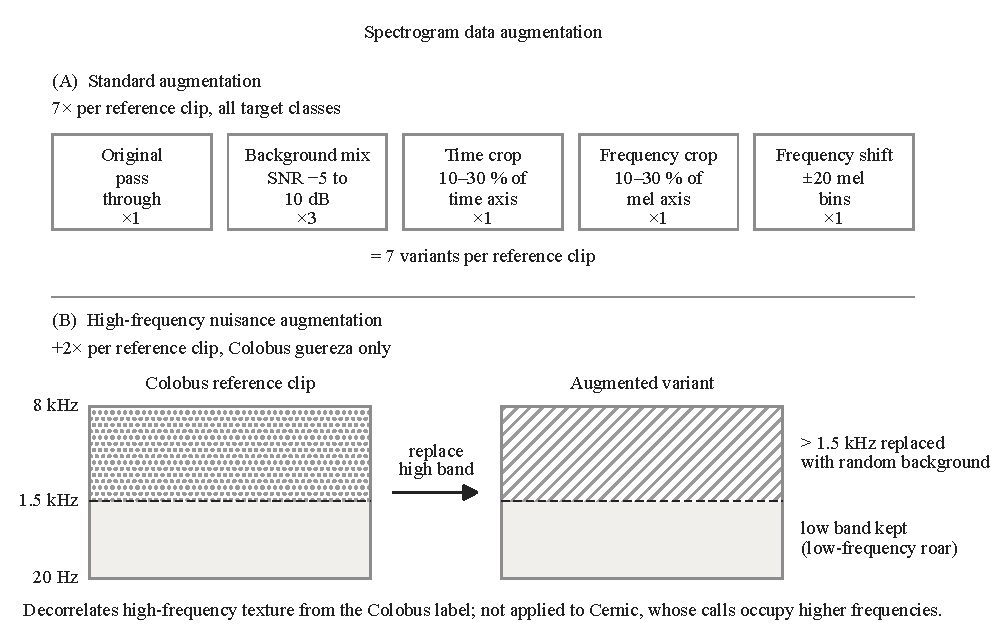
\includegraphics[width=\linewidth]{Figure_1.pdf}
\caption{Spectrogram data augmentation. (A)~Each target-class clip is expanded
by four operations, cycled until the class reaches 3{,}000 examples: a
background mix at $-5$ to 10\,dB SNR, a time crop, a frequency crop (each
5--10\,\% of the axis), and a $\pm$9-mel-bin frequency shift.
(B)~High-frequency nuisance augmentation adds two further
variants for \textit{Colobus guereza} only: the mel band above 1.5\,kHz is
replaced with the high band of a random background clip while the
low-frequency roar is kept, decorrelating high-frequency texture from the
\textit{Colobus} label.}
\label{fig:augmentation}
\end{figure}

\subsection*{Model architecture}

The classifier couples a VGG19 convolutional backbone \cite{simonyan2015}
pretrained on ImageNet \cite{deng2009} with a custom temporal-frequency CRNN
head (Fig.~\ref{fig:architecture}) designed to exploit both the spectral
location and the temporal rhythm of primate calls. The motivation is that Colobus roars concentrate energy around
$\sim$512\,Hz, putty-nosed calls around $\sim$1\,kHz, and common confusers
(birds, insects) above $\sim$2\,kHz; encoding where in frequency the
energy sits and when it occurs lets the model discriminate species that
a global pooling layer would conflate.

The feature map from block4\_conv4 of VGG19 (spatial size
28\,$\times$\,28, 512 channels) is extracted before the final VGG19 block.

\paragraph{Frequency-position encoding.}
VGG19's convolutions are translation-invariant along both image axes, including
frequency: a rhythmic, harmonically structured call texture produces almost the
same feature response whether it sits low in the spectrogram (a \textit{Colobus}
roar) or high (a bird trill or insect chorus). A head that pools or convolves
these features therefore keys on the call texture while discarding
where in frequency it occurred, exactly the cue a human uses to tell a
low roar from a high bird call. To restore this information we append an
explicit frequency-coordinate channel to the feature map: a normalized
``CoordConv'' channel \cite{liu2018} whose value runs from 0 at the lowest
mel-frequency row to 1 at the highest, constant across time. A
Conv2D(128, kernel 3, same padding) + batch normalization + ReLU then fuses this
coordinate with the texture channels, so every downstream feature is tagged with
the absolute frequency at which it occurs. The network can then learn that a
given call texture means \textit{Colobus} only when it appears at low frequency,
and reject the same texture higher up.

The frequency axis (height) of the resulting 28\,$\times$\,28\,$\times$\,128
feature map is then split into four equal bands (each 7 bins), so that
each band covers a contiguous portion of the mel-frequency range. Within each
band, the frequency dimension is collapsed (average pooling over the 7 bins),
yielding a time-$\times$-channel sequence of shape 28\,$\times$\,128. Each
band is then processed by its own one-dimensional convolutional stream:
Conv1D(128 filters, kernel size 3, same padding) followed by batch
normalization and ReLU, producing four sequences of shape
28\,$\times$\,128. These are concatenated along the channel axis
(28\,$\times$\,512) and passed through a cross-band Conv1D(256, kernel 3,
same padding) + batch normalization + ReLU layer that allows the network to
learn interactions between frequency bands.

The resulting 28\,$\times$\,256 sequence is fed into a bidirectional LSTM with
128 units per direction (return sequences enabled, input dropout 0.3),
which captures temporal dependencies such as the rhythmic hack--hack or
pyow--hack patterns characteristic of putty-nosed calling bouts. The LSTM
output sequence is summarized by concatenating global max pooling and global
average pooling over the time axis, producing a 512-dimensional vector that
retains both peak activation and average energy. This vector passes through
two dense layers (512 units, ReLU, dropout 0.5; then 256 units, ReLU, dropout
0.5) and a final softmax over the trained classes. The deployed model has four
(Cernic, Colobus\_guereza, Colobus\_confuser, Background); the retrained heads
evaluated in Table~\ref{tab:loso} have five, the fifth being \textit{C.\
pogonias} for the reasons given under Limitations. Both were read from the saved
graphs rather than from the configuration file, which records only the current
setting and would have reported five for each.

\begin{figure}[H]
\centering
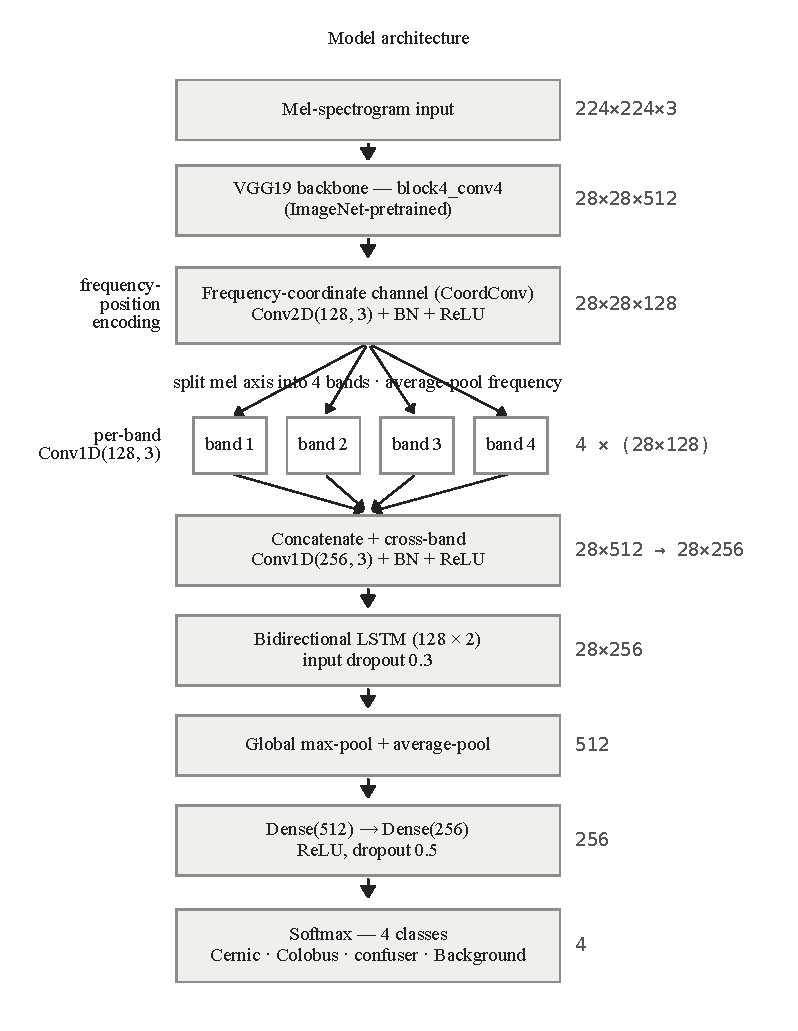
\includegraphics[width=0.82\linewidth]{Figure_2.pdf}
\caption{Model architecture. A VGG19 backbone (the block4\_conv4
feature map) is augmented with a frequency-coordinate (CoordConv) channel, then
split into four mel-frequency bands processed by per-band and cross-band 1-D
convolutions, summarized by a bidirectional LSTM with combined global max- and
average-pooling, and classified by two dense layers and a softmax --- drawn here
with the deployed model's four outputs; the retrained heads add a fifth for
\textit{C.\ pogonias}. The
frequency-position encoding and the per-band split are the components added to
suppress \textit{Colobus} false positives. Output tensor shapes are shown on
the right.}
\label{fig:architecture}
\end{figure}

\subsection*{Model training}

Training proceeds in two stages, following a standard transfer-learning
protocol of head training followed by partial fine-tuning.

\paragraph{Stage 1: Head training.}
The entire VGG19 convolutional base is frozen and only the temporal-frequency
CRNN head is trained. The optimizer is Adam with an initial learning rate of
$1 \times 10^{-4}$, and the loss is sparse categorical cross-entropy.

\paragraph{Stage 2: Partial fine-tuning.}
Because the VGG19 base is truncated at block4\_conv4
(\S\,Model architecture), its trainable portion spans blocks 1--4. The last two of these
blocks (the block3 and block4 convolutional layers) are
unfrozen, while block1 and block2 remain frozen to preserve
low-level features; this makes $\approx$12.3\,M parameters trainable. The
learning rate is reduced to $1 \times 10^{-5}$ to avoid catastrophic
forgetting.

\paragraph{Shared training settings.}
Both stages use the augmented dataset split 80/20 into training and validation
sets with stratification by class and a fixed random seed for
reproducibility. Balanced class weights (inversely proportional to class
frequency) compensate for the larger Background class. Training runs for up to
50 epochs per stage with a batch size of 32, governed by three callbacks:
early stopping on validation loss (patience 10, best weights restored),
model checkpointing on best validation accuracy, and learning-rate reduction
on plateau (factor 0.5, patience 5, floor $1 \times 10^{-7}$). The best
checkpoint is saved. Training concludes with a
per-class accuracy report and a confusion matrix on the validation set.

\subsection*{Sliding-window detection}

A trained model is applied to each long recording with a 2.0\,s window
advanced in 1.0\,s steps (50\,\% overlap); a final window is anchored at the
end of the file so trailing audio is not dropped. Every window is converted to
a mel-spectrogram image and classified. The four softmax classes are first
collapsed onto detection groups: the
putty-nosed call types are already merged into Cernic at training time, so
Cernic and Colobus\_guereza map to themselves, while the Colobus\_confuser
class is routed into the Background group. Summing the confuser probability
into Background means a window the model calls ``confuser'' is excluded from
detections exactly like Background, and, equally important, the confuser
probability is kept out of the Colobus\_guereza group, so a genuine
\textit{Colobus} window is no longer inflated by confuser energy. The window is
assigned to its highest-scoring group and is kept as a detection if that group
is not Background and its confidence meets a threshold (default 0.4).
Overlapping detections of the same group are then reduced by per-class
non-maximum suppression at an intersection-over-union threshold of 0.5.

\paragraph{Low-frequency energy gate for \textit{Colobus}.}
After NMS, a frequency-domain safety net is applied to each remaining
\textit{Colobus} detection. A short-time Fourier power spectrum of the 2\,s
clip is computed with the same FFT size and hop length as the mel front end,
and within the 20--8000\,Hz analysis band the fraction of energy that falls
below 1.5\,kHz is measured. Genuine \textit{Colobus} roars concentrate almost
all of their energy in the low band and sit well above the gate threshold,
whereas the high-frequency bird and insect sounds that the classifier
occasionally mis-fires on carry almost all of their energy above 1.5\,kHz.
Detections whose low-frequency ratio falls below the threshold are dropped from
the detection list (i.e.\ treated as non-target Background).

The deployment reported here used a threshold of 0.20. That value was
calibrated on the curated \textit{Colobus} reference clips together with the
\textit{Colobus\_confuser} training clips, whose low-frequency ratios do not
exceed 0.09; 0.20 therefore sat in a wide empty gap and retained 97.6\,\% of
the reference clips. The calibration did not survive contact with the field.
Of the 253 \textit{Colobus} detections the deployment returned, \emph{none}
has a low-frequency ratio below 0.20 (minimum 0.2007, median 0.4231, upper
quartile 0.8365, maximum 0.9831), so the gate removed none of them. The
dominant field confuser is not a high-frequency insect or bird but thunder,
which is itself low-frequency and therefore passes the gate by the same
criterion that admits a roar. The repository now sets the threshold to 0.40
(\texttt{LOWFREQ\_GATE\_THRESHOLD}, \texttt{src/config.py}), which retains
93.4\,\% of the reference clips and 133 of the 253 field detections
(52.6\,\%). The gate should be read as a partial mitigation against one
high-frequency confuser, not as a control on the \textit{Colobus} false
positives actually observed. The low-frequency ratio is also written as a column
in the output CSV for every retained detection, so detections can be ranked or
re-inspected by it.

Per-file detections (start time, end time, species, confidence) are written to
CSV, and a short waveform clip around every detection is exported so that
review and downstream filtering do not require re-reading the long recordings.

\subsection*{Automatic false-positive cleanup}

The detector's raw output contains many false positives from sounds absent
from the training set. Three independent filters, each exploiting a different
signal, are run over the saved detections; their agreement determines how a
detection is treated. For each detection a 2\,s clip is extracted from the
source recording. The same per-detection signals are then reused to group and
order the remaining detections for manual review, which is where most of the
practical saving turns out to lie.

\paragraph{(a) Mahalanobis out-of-distribution filter}
Using a penultimate dense layer as a feature extractor, per-class feature means
and a pooled, ridge-regularized inverse covariance are estimated from the
original (non-augmented) training clips \cite{lee2018}. For each detection the
Mahalanobis distance to its candidate class cluster is computed. A real call
lies close to its training cluster, whereas an unfamiliar sound does not.
Because field clips are systematically noisier than the curated training clips,
thresholds calibrated on training data flag almost everything; we therefore
calibrate the cutoff on the \textbf{detection distances themselves}, flagging,
per species, the detections beyond the 95th percentile of the observed
distance distribution (a configurable percentile). This makes the filter a
relative-outlier detector that is robust to the train-to-field domain shift.

\paragraph{(b) YAMNet cross-check (implemented, disabled)}
The pipeline also implements a cross-check against YAMNet, a network trained on
Google's AudioSet ontology \cite{gemmeke2017,hershey2017}, flagging a detection
whose top class is a non-primate sound. It is off by default: AudioSet has no
monkey-specific class, and the field review showed it labels putty-nosed calls
with the same classes as the surrounding forest, so it flagged more genuine
calls than false positives. It is described here because the code retains it
for targets that AudioSet does represent.

\paragraph{(c) Temporal-isolation filter}
Primates tend to call in bouts, so a genuine call usually has same-species
neighbours nearby in time. A detection with no other detection of the same
species within $\pm$30\,s (configurable) is flagged as temporally isolated.

A detection is considered \textbf{clean} only when no filter flags it,
\textbf{suspicious} when at least one filter flags it, and a \textbf{strong
false positive} when at least two filters agree. Clean and suspicious
detections are written to separate CSVs (the suspicious file carries a
human-readable flag-reason column), and strong false positives are
exported as labelled WAV clips for the next stage.

\subsection*{Organising the review: episodes and ordering}

Discarding a detection is only one thing that can be done with these signals,
and on our field data it turned out to be the least useful (see
\S\,Method validation). Two further steps use the same per-detection
information to reduce how much listening the surviving detections cost, without
removing any of them. Both are parameter-free in the sense that matters here:
neither fits a cutoff on labelled data, so neither can fail to transfer to a
new site.

\paragraph{(i) Grouping detections into listening episodes}
Detections of one species in one recording that fall within a fixed gap of each
other (five minutes by default) are grouped into an \textbf{episode}. An
episode is the unit a reviewer actually decides on: a non-target sound that
runs for a stretch of a recording produces many detections, and hearing one of
them settles the whole stretch. Review effort is therefore counted as one
listen per episode that turns out to be uniformly non-target, and per clip only
within episodes that mix genuine calls with false positives. Nothing is
discarded and no threshold is involved; the grouping only changes how the same
detections are presented.

\paragraph{(ii) Ordering the review by averaged within-station ranks}
The clips that still need listening are presented most-likely-genuine first.
Four signals the pipeline already computes are used: the detector's confidence,
the margin between its top two class scores, the number of same-species
detections within the temporal-isolation window, and the Mahalanobis distance
(entered with its sign reversed, since large is bad). Each is converted to a
percentile rank \emph{within its own station}, and the four ranks are averaged
into one score. Ranking within the station is what makes this robust: the raw
scales of these signals differ between sites, which is exactly why fixed
cutoffs transfer badly, but a percentile rank is scale-free by construction.
No weights are fitted and no cutoff is chosen --- the reviewer simply stops when
their budget runs out, and the ordering is reported as an average precision,
which summarises every possible stopping point at once.

\paragraph{(iii) Consolidating overlapping windows into call events}
At a finer scale than an episode, consecutive windows on one vocalization are one
sound. Because the window advances in steps shorter than itself, and because
non-maximum suppression is deliberately set to keep neighbouring windows so that
a boundary-straddling call is not lost, a call longer than one step is reported
more than once. Detections of one species in one recording whose windows overlap
or touch are therefore also grouped into a \textbf{call event}, and the pipeline
reports the event count beside the window count. The distinction matters for two
different readers: review effort is paid per window, but vocal activity is a
count of events, and only the latter is comparable across studies with different
window settings. Like the two steps above, this is grouping by timestamp, with
nothing discarded.

\paragraph{What the reviewer receives}
Both steps are label-free, so the pipeline emits them directly rather than
leaving them to a later analysis: the cleanup writes a review queue over
\emph{all} detections, before the clean/suspicious split, holding one row per
detection in the order described above and one row per episode marked as the
clip to listen to first. It is written in the column layout of the annotation
software used here (Kaleidoscope Pro) with the manual-identification field left
blank, so a reviewer works down the file and fills it in. Reading the queue
top-down does two things at once: genuine calls surface early, and the long runs
of non-target sound collect at the end, where each is met as a block and settled
in one listen.

\subsection*{Iterative hard-negative mining}

The exported strong false positives are the sounds the detector most needs to
learn to ignore. They are added to the Background class and the model is
retrained from the preprocessing stage, so that on the next pass the network
is far less likely to fire on those sounds. Repeating the detect $\rightarrow$
clean $\rightarrow$ fold-in $\rightarrow$ retrain loop a few times (typically
three to five iterations) progressively drives down the false-positive rate
without ever requiring exhaustive manual annotation of the field recordings.

When one species' false positives are dominated by a single, recurring
confuser rather than a diffuse mix of sounds, folding them into the generic
Background class is not enough: a few hundred hard negatives are easily diluted
among several thousand background clips. In that case we promote the confuser
to its own softmax class (here, Colobus\_confuser) and route it back
into the Background group only at detection time. This gives the optimizer an
explicit boundary to fit while leaving the detection behaviour unchanged, and
is the approach used for the low-frequency \textit{Colobus} confuser in the
current model. Because every field detection clip is exported during detection,
this hard-negative mining can be repeated from the saved clips even after the
source recordings have been deleted to save storage.

\subsection*{Reproducibility and reuse on new species or sites}

The complete method is released as a self-contained repository
(\url{https://github.com/mo119m/primates-sound-detection}) designed to be run by
others, not only read. Its README provides complete, step-by-step documentation,
and ready-to-run Jupyter notebooks reproduce the entire workflow --- preprocessing,
training, sliding-window detection, and the false-positive cleanup
--- with no code editing. Notebooks are provided for both running
locally (on a personal machine, with automatic use of a GPU if present and a
CPU fallback otherwise) and running in the cloud on Google Colab with a free
GPU, so users can choose whichever suits their hardware. The Python dependencies
are pinned so that the exact software environment used to train the released
model can be recreated on Windows, macOS, or Linux.

Crucially, the pipeline is configuration-driven: all paths, class
definitions, audio parameters, and hyperparameters live in a single
\texttt{config.py}. Re-targeting the method to a different species or field site
requires no change to the source code. A user drops their own labelled reference
clips into the \texttt{data/} folders, lists the new class names in the
\texttt{SPECIES\_FOLDERS} and \texttt{BACKGROUND\_FOLDERS} dictionaries, and
re-runs the same notebook; the number of output classes, class weighting, and
the detection grouping all follow automatically from that configuration. The
frequency-position head, confuser-class mechanism, and cleanup filters are
generic and apply unchanged to any new target call. In this way the repository
functions both as an exact reproduction of the results reported here and as a
reusable template for new passive-acoustic-monitoring problems.

%% =====================================================================
%% METHOD VALIDATION -- data that validate the method (no Results/Discussion).
%% =====================================================================
\section*{Method validation}

We report validation at two levels: (i) performance on a held-out validation
split drawn from the same curated clip pool as training, and (ii) deployment on
the continuous field recordings, where the biology of the site provides an
independent check on the \textit{Colobus} false-positive rate.

\paragraph{Validation-set performance (V12 model).}
The four-class V12 model (the frequency-position-aware head with
high-frequency nuisance augmentation) was evaluated on a stratified
validation split. The model was trained in two stages
(Fig.~\ref{fig:training}): a frozen-base stage that trains only the
classifier head, followed by a fine-tuning stage in which the last two VGG19
blocks are unfrozen. Both stages use early stopping and learning-rate
reduction on a validation-accuracy plateau.

\paragraph{We do not report a validation accuracy, and the reason is a result.}
Earlier versions of this manuscript reported 98.12\,\% overall accuracy on a
stratified validation split, with per-class figures and a confusion matrix whose
cross-species off-diagonal was zero. Those numbers measured memorisation and
have been withdrawn. The split was taken \emph{after} augmentation: with an
augmentation multiplier of seven, a source clip keeps all of its variants on one
side of an 80/20 split only $0.8^{7} = 21\,\%$ of the time, so roughly 79\,\% of
source clips placed a near-duplicate of a validation image into training. The
\textit{Colobus} class was worse again, its windows cut at a 1\,s hop so that
neighbours share half their audio before augmentation is applied at all. The
distance between that 98\,\% and the 41.0\,\% field precision reported in
\S\,Field deployment is the size of what the split was hiding.

The zero cross-species confusion deserves a separate warning, because it is the
kind of number that survives into abstracts. It was not evidence that the model
separates the two species. Every \textit{C.\ guereza} training clip is archival
library media and every \textit{C.\ nictitans} clip was recorded at the study
site, so that cell separated two recording channels, not two animals.

The immediate remedy is to split on the source recording rather than on the
image, so that no clip and no augmented variant of it can appear on both sides
(\texttt{train.grouped\_split}); in the dataset as it stood at that point the
617 \textit{Colobus} windows collapsed to their 172 source recordings and the
17\,106 archival segments to 3\,222, and
a simulation that reproduces 79\,\% leakage under the original split yields
none. Doing that raises the honest question rather than answering it. Under the
grouped split the same architecture reaches 95.8\,\% mean validation accuracy
across the sixteen folds reported below, but the validation set is 85.7\,\%
Background, so answering Background to everything scores 85.7\,\%, and the
model's real margin over doing nothing is about ten points. More importantly,
any validation split is drawn from the same curated pool the model was trained
on, and the deployment is not. We therefore replace the validation table with a
field measurement on stations the model has never heard
(Table~\ref{tab:loso}), and recommend that reuse of this pipeline be judged the
same way. A curated-pool accuracy, honestly split or otherwise, did not predict
what happened in the forest.

That recommendation needs one qualification, which we can make because we later
tested it on ourselves. Table~\ref{tab:loso} is a better measurement than
validation accuracy, but it is still a \emph{re-ranking} measurement: it scores
a model on the candidate list some other model produced. Under Limitations we
report configurations whose held-out precision differs by 0.81 at one station
and which recover exactly the same calls when run over raw audio, and
configurations whose held-out precision differs by 0.002 at another station and
which do not. Held-out re-ranking precision is therefore not a proxy for
scanning behaviour in either direction, and a reader choosing between two models
on the strength of Table~\ref{tab:loso} alone may be choosing on noise. The
measurement that separated them was a scan of raw audio at a held-out station
with the results checked by ear. It is more expensive than either table in this
paper, and on this evidence it is the one that decides anything.

\begin{figure}[H]
\centering
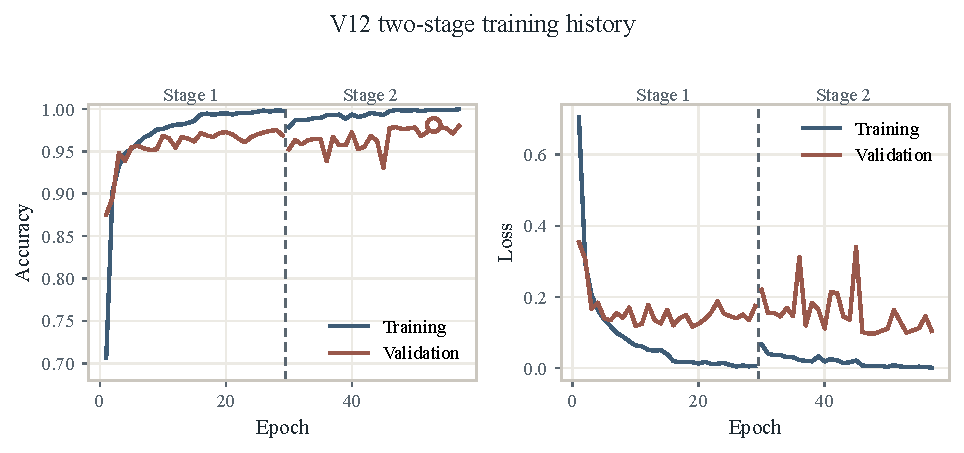
\includegraphics[width=\linewidth]{Figure_3.pdf}
\caption{Two-stage training history of the V12 model: training and validation
accuracy (left) and loss (right) per epoch. The dashed line marks the
transition from frozen-base head training (Stage~1) to fine-tuning of the last
two VGG19 blocks (Stage~2). The deployed model is the checkpoint with the
highest validation accuracy. The validation curve itself is drawn from a split
taken after augmentation and is therefore optimistic throughout; it is shown to
document the training procedure, not to quantify performance
(\S\,Model training).}
\label{fig:training}
\end{figure}








\noindent One design element does survive the withdrawal of those numbers,
because it is a routing decision rather than a performance claim: the dedicated
confuser class is folded into the Background group at detection time
(\texttt{config.DETECTION\_GROUPS}), so a window the model assigns to it cannot
produce a \textit{Colobus} detection. That is a property of how the softmax is
read, not something a validation split establishes.

\paragraph{Field deployment.}
The V12 model is run on the continuous recordings from all available acoustic
stations; one 2\,s clip is exported for every detection that survives the
low-frequency energy gate. As an architecture-level check during development,
the position-aware head (with the frequency-position encoding) was compared
against the earlier position-blind head on a set of \textit{Colobus} detection
clips: of six high-frequency bird false positives that the position-blind head
had labelled \textit{Colobus}, the position-aware head reclassified
five as Background or confuser while preserving all genuine \textit{Colobus}
reference clips at full confidence, confirming that the frequency-position
encoding suppresses the high-frequency confusion rather than trading away true
positives. The final (V12) model adds the high-frequency nuisance augmentation
and the calibrated low-frequency gate on top of this encoding and is the
version deployed across all stations.
%% ---------------------------------------------------------------------
%% FIELD-DEPLOYMENT RESULTS -- every figure below comes from
%%   data/outputs/auto_cleanup/cleanup_vs_review.csv
%% which is in the repository and carries one row per reviewed detection with
%% the reviewer's verdict and every cleanup signal. That file is the ground
%% truth for this section; it is what to cite and what to re-run against.
%%
%% The raw per-station Kaleidoscope exports (reviews/, gitignored) are NOT
%% needed to reproduce anything here. They were checked: their MANUAL ID column
%% holds the single value "Noise" for all 3 654 false positives, so the merge
%% into the file above discarded nothing. summarize_review.py still reads them
%% if you have them locally.
%% The review covers C. nictitans only; see the scope sentence below.
%% ---------------------------------------------------------------------
The final (V12) model was deployed across 16 acoustic stations. This section
reports the \textit{Cercopithecus nictitans} detections, every one of which was
verified by ear. The same run produced 253 \textit{Colobus guereza} detections
(median confidence 0.953). All 253 were subsequently verified by ear and
\emph{none} is a genuine roar: field precision for that class is 0.0\,\%, and
because the field record therefore contains no confirmed positive, field recall
for \textit{C.\ guereza} is not estimable from these data. We report this as a
negative result; \S\,Limitations discusses what it does and does not license.

\paragraph{The \textit{Colobus} detections are spatially impossible for one
animal.} A verdict that rests on listening rests on one person's ears. The array
supplies an independent test that does not. AudioMoth writes the deployment
lat/lon into every filename, which recovers coordinates for 11 of the 16
stations, a grid spanning 6.68\,km at its widest and 2.49\,km between a
median pair. A guereza roar carries about 1.6\,km, so two recorders that both hear the
same calling animal cannot be more than roughly 3.2\,km apart. Whether a group
of near-simultaneous detections could have come from a single source is then
arithmetic rather than judgement.

Grouped into five-minute slots, \textbf{61.5\,\% of the \textit{Colobus}
detections fall in slots spanning more than 3.2\,km}, against \textbf{24.0\,\%
for \textit{C.\ nictitans}}, a species confirmed present, which is what makes it
the control that decides whether the test measures anything at all. The two
largest \textit{Colobus} slots are 2021-02-24 15:10, seven stations across
4.73\,km, and 19:30 the same day, five stations across 4.41\,km.

The control needs stating precisely, because the obvious description of it is
the wrong one. Across the eleven stations with coordinates the test uses 3\,011
\textit{C.\ nictitans} detections and 156 \textit{Colobus} detections, and it
selects them by predicted species alone. It does not consult the review
verdicts, so 981 of those 3\,011 are detections a reviewer has confirmed are
\emph{not} \textit{C.\ nictitans}; only 2\,029 are confirmed calls. Both
populations are worth reporting, and they do not agree. Restricting the control
to the 2\,029 confirmed calls lowers it at every slot width --- false positives
are more spatially dispersed than real choruses, which is the same signal the
test is built on --- and therefore widens the gap the test reports rather than
narrowing it.

The choice of a five-minute slot is not free, and the sweep across slot widths
is the result rather than a robustness check:

\begin{center}
\begin{tabular}{lrrrr}
\toprule
 & & \multicolumn{2}{c}{\textit{C.\ nictitans} control} & \\
\cmidrule(lr){3-4}
Slot width & \textit{Colobus} & all detections & confirmed calls & Difference \\
\midrule
30\,min & 71.8\,\% & 74.8\,\% & 32.8\,\% & $+39.0$ \\
15\,min & 63.5\,\% & 52.2\,\% & 20.7\,\% & $+42.7$ \\
\textbf{5\,min} & \textbf{61.5\,\%} & \textbf{24.0\,\%} & \textbf{8.3\,\%} & $\mathbf{+53.2}$ \\
1\,min & 35.9\,\% & 8.0\,\% & 4.6\,\% & $+31.3$ \\
30\,s & 1.3\,\% & 5.6\,\% & 3.6\,\% & $-2.3$ \\
15\,s & 0.0\,\% & 3.8\,\% & 2.6\,\% & $-2.6$ \\
\bottomrule
\end{tabular}
\end{center}

\noindent Difference is against the confirmed-call control. Against all
detections the five-minute gap is $+37.5$ and the thirty-minute gap is $-3.0$;
the choice of control changes the size of the effect at every width and its sign
at thirty minutes, which is why both columns are shown.

Five minutes is where the two mechanisms are furthest apart under either
control. What the coarse end shows depends on which control is used: against all
detections the two species are indistinguishable at half an hour, whereas
against confirmed calls a 39-point gap survives there. The conservative reading
is the first, and it is the one to rely on --- a slot that wide pools
independent callers, and an effect that only appears once the control is
filtered is an effect that leans on the filtering. Below a minute the sign
reverses under both, and that reversal is the
informative half: a genuine chorus does reach neighbouring recorders within
seconds, so \textit{C.\ nictitans} rises, while the \textit{Colobus} detections
do not, because thunder rolls and rain arrives progressively and a front is
minutes wide rather than seconds wide. Five minutes is also the crossing time of
a squall over an array this size. Reproduce with
\texttt{scripts/spatial\_extent\_test.py -{}-sweep}; the confirmed-call column
additionally requires joining the detections to the review table on site and
detection time.

This does not identify what the detector fired on; it establishes that most of
it cannot have been one animal, using geometry, a published carrying distance
and a positive control, and not an ear.

\paragraph{Two targeted searches of the raw audio, and what they found instead.}
A detector that never fires on a species establishes nothing about the species
until you have looked for it another way. We therefore searched the raw
recordings twice more, choosing the search windows from the published behaviour
rather than from the deployment: guereza roaring bouts occur mainly at night and
at dawn, and a roaring phrase is about fifteen pulses of roughly 0.7\,s -- a
1.4\,Hz pulse train sustained for some ten seconds, a temporal signature that
thunder, a single decaying transient, cannot produce.

The first search scored every 2\,s window of the dawn period, 05:00--08:00, at
all 16 stations: 390 recordings, 194\,h, 698\,007 windows
(\texttt{scripts/colobus\_dawn\_probe.py}). Rather than thresholding, we recorded
the score distribution, because a threshold chosen elsewhere returning nothing
is indistinguishable from an absent animal. 124 windows exceeded 0.10 on the
\textit{Colobus} output. Of those, 117 have more than 95\,\% of their energy
above 1.5\,kHz and cannot be a low-frequency roar whatever the model says; the
strongest of them scores 0.9995 with a low-frequency ratio of 0.010. The
remaining seven come from a single recording and were listened to: they are real
animal vocalisations, low and guttural, and not \textit{C.\ guereza}.
\textit{C.\ nictitans} was scored on the same audio in the same forward pass as a
positive control and returns confident detections in 84 of the 390 recordings,
so the silence is a property of the \textit{Colobus} channel and not of the
pipeline.

The second search dropped the classifier entirely and looked for the pulse train
directly in 630\,h of night audio, 19:00--05:00, 1\,269 recordings, 453\,677
windows (\texttt{scripts/scan\_roar\_pulse.py}). This has the advantage of not
depending on a model whose every \textit{Colobus} training example is archival:
it asks a question about the audio instead. Only 57 of the 1\,269 recordings
contain any window at all in which low-frequency energy dominates. Ranking those
by the strength of 1--2\,Hz amplitude modulation and listening to the top ten:
every one is a bird. The feature works: it recovered the most strongly
periodic low-frequency vocalisations in the corpus, and none of them is a
roar.

Four independent lines therefore agree, and their agreement is the result:
the deployment's own 253 detections (none genuine), the dawn model search (no
plausible candidate), the model-free night search (birds), and the spatial test
above (61.5\,\% of detections unreachable by a single source). Across roughly
1\,000\,h of audio and four methods that do not share a failure mode, no
acoustic evidence of \textit{C.\ guereza} was recovered at this site.

Two limitations bound all of it. First, a roar at the edge of its 1.6\,km range
arrives faint and may not retain measurable periodicity, so absence of evidence
here is weaker than it looks, because the searches would miss a distant animal.
What they do establish is that no near or mid-range roaring bout occurred in the
periods searched, which for a species whose males roar to advertise territory is
the period in which one would expect to find them.

Second, and more restrictive, the result is about \textit{C.\ guereza} only.
\textit{C.\ satanas} also has range covering this area~\cite{iucnsatanas2020}
and the two vocalise very differently, so nothing here bears on whether the
black colobus is present: every reference clip the detector was built from is
\textit{C.\ guereza}, and the pulse-train criterion was derived from published
descriptions of the \textit{C.\ guereza} roar. A search for \textit{C.\ satanas}
would need its own reference material and its own acoustic criterion, and would
be worth doing: the acoustic literature for that species comes almost entirely
from Lopé National Park, several hundred kilometres to the southwest.

\paragraph{A positive control, and how far it resolves the null.}
A null from a detector admits two readings: the animal did not vocalise, or the
detector cannot recognise it under field conditions. Separating them requires a
positive control, a recording in which the species is known by ear to be calling,
scored by the same detector. For most of this work none was available. Every
\textit{C.\ guereza} clip in the training set is archival library media, and no
field-verified roar was known to the species expert consulted here.

One became available after the analysis above was complete. The expert supplied
nine three-second clips of black-and-white colobus, verified by ear and cut from
an independent passive-acoustic deployment: a different recorder, a different
forest, and a project unconnected to this one. They are field recordings in the
sense that matters here, ambient passive units in humid forest, which is the
recording channel this detector was suspected of failing on. Each clip also
carries the confidence its own project's detector had assigned to it, which
turns out to be informative.

Scored by the classifier described above, the \textit{Colobus} output reaches
0.5 on three of the nine, at 1.0000, 1.0000 and 0.9963. The \textit{C.\
nictitans} output stays at or below 0.0025 on all nine, so the response is
specific to the class rather than a general reaction to loud low-frequency
sound. The three that fire are all drawn from the five clips the originating
detector had scored at 1.000; of the four it scored between 0.903 and 0.917,
none exceeds 0.0001 here. Taken at face value that is a per-clip recall of three
in nine. Restricted to the subset the originating detector was itself certain
of, it is three in five, and the two misses in that subset returned 0.0138 and
0.0378.

Two limits bound what those figures mean. The nine clips are not a random sample
of guereza vocalisations but calls that another detector had already flagged, so
the recall describes agreement on calls that were detectable to begin with
rather than recall over everything the animal produces. Nine clips also cannot
support a precise estimate of either quantity.

What they do support is the reading of the null. The detector responds to
\textit{C.\ guereza} in passive field audio, and when it responds it does so at
full confidence rather than marginally. The absence of a single confirmed roar
in 630 hours is therefore better explained by the species not calling within
range of these stations than by a detector unable to cross from archival to
field recordings. That is a reduction of the ambiguity and not its removal: a
detector missing more than half of the calls another detector found can still
miss a rare caller, and sixteen stations sample a small part of a large forest.
Readers holding further confirmed roars can extend the test with
\texttt{scripts/colobus\_dawn\_probe.py} and
\texttt{scripts/scan\_roar\_pulse.py}.

The contrast with \textit{C.\ nictitans} remains instructive. That species had
2\,535 field-verified calls behind it, and every claim made about it here is
testable against them. \textit{C.\ guereza} has nine, obtained late and from
elsewhere, which is enough to interpret a null and not enough to characterise a
detector.
The model produced 6\,189 \textit{C.\ nictitans} detections across the 16
stations, of which 2\,535 were confirmed as genuine calls and 3\,654 were
non-target forest sounds, an overall precision of 41.0\,\%
(Table~\ref{tab:field}).

That aggregate is dominated by a single station. IPA4ST alone produced 2\,470
detections --- 40\,\% of all detections --- of which only 100 were genuine
(precision 4.0\,\%), contributing 2\,370 of the 3\,654 false positives. Across
the remaining fifteen stations precision was 65.5\,\% (2\,435 confirmed of
3\,719), and the median per-station precision was also 65.5\,\%, ranging from
20.8\,\% at IPA11ST to 93.1\,\% at IPA20ST. Listening to IPA4ST's detections
identified the cause: a non-target species abundant at that station and absent
from the training data. It is treated separately below, because it is the one
case that none of the per-detection cleanup signals can read.

One point of interpretation applies to all of these counts. Detection advances a
2\,s window in 1\,s steps, and per-species non-maximum suppression removes only
windows overlapping by more than half, so two consecutive windows --- which
overlap by a third of the time they jointly span --- both survive, deliberately,
so that a call straddling a boundary is not lost. A vocalization longer than the
1\,s step is therefore reported by more than one window, and the figures above
count \emph{windows}, not calls. They are the right unit for precision, which is
a property of what the detector reported, and for review effort, which is paid
per clip; they overstate vocal activity, and the pipeline therefore also
consolidates consecutive windows into call events
(\S\,Automatic false-positive cleanup) and reports both counts. Consolidated,
the 6\,189 windows are 2\,103 call events and the 2\,535 confirmed windows are
\textbf{755 confirmed \textit{C.\ nictitans} vocalizations}: a window count
overstates vocal activity here by a factor of 3.36. Any use of these data as a
measure of calling activity should use the event counts.

\subsection*{Leave-one-station-out validation}

Because a validation split of any kind is drawn from the same curated pool the
model was trained on, the only measurement that speaks to deployment is one
taken on a station the model has never heard. We therefore retrained the
classifier sixteen times, once per station, each time withholding every
training clip that could have come from that station and scoring only that
station's reviewed detections (\texttt{scripts/train\_v13\_loso.py}). Station
attribution is not optional here: eleven stations stamp a unique lat/lon into
each filename, but IPA1, IPA2, IPA4, IPA6 and IPA7 recorded with GPS disabled
and write identical names, so the 1\,008 clips that could belong to any of them
sit out every fold they might contaminate. The sixteen held-out folds partition
the 6\,189 reviewed detections exactly.

Scoring is restricted to the recalibrated deployment window 05:00--19:00
(\S\,Sliding-window detection), which retains 3\,571 of the 6\,189 detections
and 2\,503 of the 2\,535 confirmed calls.

The operating point is the part of this design that is easiest to get wrong, so
it is stated explicitly. A threshold chosen to retain a fixed share of the
held-out station's own confirmed calls compares the two models at equal recall,
which is the right question when asking whether the retrained model \emph{ranks}
calls above false positives better. It is not an operating point. Choosing it
needs the answers, and across the sixteen folds the value that retains 95\,\% of
the calls ranges from 0.0024 to 0.9953, so no single number of that kind could be
handed to anyone. Table~\ref{tab:loso} therefore reports a threshold fitted the
way a practitioner would fit one: on the reviewed detections of the other fifteen
stations, then applied unchanged to the held-out sixteenth, under the same
grouped-argmax rule the deployment uses. Recall becomes a measured outcome
instead of a constraint, which is why the calls-kept column varies.

\begin{table}[H]
\centering
\caption{One round of review-and-retrain, one fold per acoustic station,
ordered by the precision of the deployed model. All figures are inside the
05:00--19:00 detection window.

\textbf{This is not a held-out precision.} Each fold withholds the station's
confirmed \emph{calls}, which need an expert and which a new site does not
have. It does not withhold the station's Background, because collecting
negatives from a site's own rejected detections is a step in this method rather
than a leak in its measurement: a user deploys, rejects the false positives by
ear, and feeds them back. Anyone running the pipeline at a new site has that
site's rejected detections before the second round, so a fold that withholds
them measures a situation no user is in. The figure below is therefore what one
round of that loop buys at a station, and it must not be read as transfer to a
station never heard.

The threshold is fitted on the fifteen other stations to retain 95\,\% of their
calls and applied unchanged to the sixteenth, so the calls-kept column is an
outcome rather than a constraint. Stations are averaged unweighted, so the
macro-average estimates a \emph{typical} station rather than the pooled corpus.
$^\dagger$The threshold row is the median, and its spread matters more than its
centre: the same rule gives 0.063 to 0.927 depending on which station is held
out, thirteen of sixteen below 0.9 and six below 0.5. No single value can be
carried to a new site.
Run provenance: \texttt{loso16.csv} in
\texttt{data/outputs/v13\_runs/allbg\_2026-08-18} --- sixteen folds complete,
15 epochs at patience 3, \texttt{--keep-all-background}, five classes, seed 42,
21\,120 training rows.}
\label{tab:loso}
\begin{tabular}{lrrrrrr}
\toprule
Station & Detections & Deployed prec. & Threshold & Retrained prec. & FP removed (\%) & Calls kept (\%) \\
\midrule
IPA1ST & 276 & 0.438 & 0.847 & 0.980 & 98.7 & 82.6 \\
IPA11ST & 93 & 0.452 & 0.804 & 0.902 & 92.2 & 88.1 \\
IPA16ST & 314 & 0.583 & 0.676 & 0.928 & 90.1 & 91.8 \\
IPA8ST & 249 & 0.619 & 0.927 & 0.987 & 97.9 & 96.1 \\
IPA19ST & 188 & 0.633 & 0.244 & 0.944 & 89.9 & 99.2 \\
IPA14ST & 236 & 0.661 & 0.455 & 0.979 & 96.2 & 89.1 \\
IPA7ST & 101 & 0.683 & 0.621 & 0.883 & 78.1 & 76.8 \\
IPA4ST & 131 & 0.695 & 0.451 & 1.000 & 100.0 & 93.4 \\
IPA18ST & 175 & 0.709 & 0.917 & 0.992 & 98.0 & 100.0 \\
IPA17ST & 501 & 0.723 & 0.063 & 0.984 & 96.4 & 82.3 \\
IPA13ST & 238 & 0.773 & 0.193 & 0.977 & 92.6 & 91.8 \\
IPA2ST & 76 & 0.842 & 0.749 & 0.983 & 91.7 & 87.5 \\
IPA15ST & 183 & 0.896 & 0.874 & 1.000 & 100.0 & 84.2 \\
IPA6ST & 168 & 0.899 & 0.891 & 0.974 & 76.5 & 98.0 \\
IPA10ST & 113 & 0.911 & 0.906 & 1.000 & 100.0 & 98.1 \\
IPA20ST & 434 & 0.959 & 0.423 & 1.000 & 100.0 & 92.3 \\
\midrule
\textbf{Macro-average} & --- & \textbf{0.717} & 0.713$^\dagger$ & \textbf{0.970} & \textbf{93.6} & \textbf{90.7} \\
\bottomrule
\end{tabular}
\end{table}

Precision improves at all sixteen stations, from a macro-average of 0.717 to
0.970, removing 93.6\,\% of the false positives while retaining 90.7\,\% of the
calls. The weakest fold is IPA7ST at 0.883; four stations --- IPA4ST, IPA10ST,
IPA15ST and IPA20ST --- remove every false positive they were given.

The recall column is the one to read alongside that. Because the threshold is
fitted on the other fifteen stations rather than on the station it is applied
to, recall is an outcome and not a constraint, and it is not uniform: it reaches
100\,\% at IPA18ST and falls to 76.8\,\% at IPA7ST and 82.3\,\% at IPA17ST. A
macro 90.7\,\% therefore describes a typical station and not a guarantee at any
particular one, and at the weakest fold a user reviewing at the fitted threshold
would miss close to a quarter of the calls present in their own detections.

One design choice behind these numbers is worth isolating, because it is the
one a reader is most likely to want to vary. Training on 16\,826 BirdNET-labelled
clips --- our own recordings, machine-labelled, never listened to --- was
compared against dropping them, on an identical evaluation set and with
everything else held fixed. Precision moves from 0.931 to 0.946, which sounds
like a result and is not: paired station by station that is 1.46 standard errors,
nine of sixteen folds improve, and over half the mean comes from one station.
The useful statement is the null. Removing 44\,\% of the training rows, on the
rule that nothing trains unless a person has heard it, costs no measurable
precision and 0.005 of recall. A practitioner can adopt that rule without paying
for it.

The fitted thresholds are the part of this table a reader is most likely to want
to reuse, and they do not support that. Fitting the same 95\,\% recall rule on
the fifteen other stations gives a median of 0.713 but an interquartile range of
0.444 to 0.879 and a full range of 0.063 to 0.927; thirteen of sixteen folds fall
below 0.9 and six below 0.5. No single value can be recommended as a starting
point. What the spread reflects is that the score distribution a station produces
depends on that station's own noise floor, so the number that buys 95\,\% recall
on fifteen stations is not the number that buys it on the sixteenth. The
procedure transfers; the constant does not, and running the procedure at a new
site requires labelled calls from that site. The spread is also not a fixed
property of the pipeline: a build made before augmentation and before the
negative-class screen was corrected showed thresholds clustered between 0.939
and 0.998, tight enough to suggest a constant could be recommended. That
clustering did not survive either change, which is a caution against reading a
narrow threshold distribution as evidence that one exists.

Five limits must be read with these numbers.
First, this is a \emph{precision} measurement on the windows the deployment
already fired on. It is not a recall measurement and says nothing about calls
neither model produced.

It is not a re-ranking result only. Reassembled into a whole model and run over
raw audio, the
retrained head was scanned rather than re-ranked at two stations chosen as the
extremes of Table~\ref{tab:loso}: IPA20ST, where the deployed model reaches
0.935, and IPA4ST, where it reaches 0.695. Every detection at or above 0.95 in a
stratified sample was listened to by the species expert. At IPA20ST 25 of 27
were genuine calls; at IPA4ST, 26 of 28; pooled, 51 of 55. All four errors sat
at the bottom of that band, near 0.95, and the fold-fitted threshold at IPA4ST
(0.964 in the current sweep, 0.995 in the earlier one) sits above them in both.
That last point is reported as it was observed and cannot be re-derived, for the
reason given immediately below: the per-clip verdicts were never written down.

That 51/55 is \emph{not} an estimate of precision above 0.95, though it is
tempting to read it as one. The clips were drawn by
\texttt{export\_detection\_clips.py -{}-reliability}, whose stated purpose is
even coverage of the confidence axis rather than of the detections: one draw per
equal-width confidence band, plus twenty from the top five percent. Of the 768
detections at or above 0.95 across the two stations, 73 lie in the top pool and
supplied 41 of the 55 listened clips, a 56\,\% inclusion rate, while the
remaining 695 supplied 14, a 2.0\,\% rate. Averaging two strata sampled 28:1
apart as though they were one sample estimates the precision of the top one-and-
a-half percentile and reports it as the precision of everything above 0.95; a
Wilson interval on it is invalid for the same reason. Because all four observed
errors fall in the stratum sampled at 2\,\%, design-weighting moves the estimate
substantially downward.

The repair is a new sample rather than a reweighting of the old one, for a
second reason: the verdicts were spoken, not recorded. The verdict column is
empty in all 185 rows of both listening sheets, so 51/55 cannot be reproduced
from any file in the repository. An equal-probability sample of 150 of the 768
detections (simple random without replacement, seed 20260811, design recorded in
\texttt{data/outputs/precision\_resample/DESIGN.txt}) is with the species expert;
every member has the same 150/768 chance of inclusion, which is what makes an
unweighted proportion and its interval mean what they say. \textbf{[Result and
Wilson interval to be inserted here on return; the abstract figure depends on
it.]}

The comparison between the two stations is the part worth keeping. The deployed
model's precision differs between them by 24 percentage points; the retrained
model's ear-verified scanning precision differs by 0.3. Whatever makes IPA4ST
hard for the deployed detector, the retrained head is not subject to it at high
confidence --- which is the property a method claiming to transfer to a new site
has to demonstrate, and it could not be demonstrated from Table~\ref{tab:loso}
alone, because that table scores both models on the same candidate list.

Two things still bound the claim. It is measured at $\ge$0.95 only, so it
describes what a user would review at the operating threshold rather than the
whole detection set; and it is precision, so a call the model never fires on is
invisible to it. Recall on raw audio remains unmeasured and needs an
independently annotated stretch of continuous recording, which this study does
not have.
Second, the review supplying the labels covers four consecutive days
(22--25 February 2021) and is entirely \textit{C.\ nictitans}; nothing here
generalises to other seasons.
Third, the \textit{Colobus} class contributes no evaluation positive to any of
the sixteen folds, because the field record contains none, so this table
measures nothing whatever about that species. The positive control described
above is the only evidence bearing on it, and scoring those nine clips with the
sixteen retrained heads rather than the deployed model gives a weaker response,
not a stronger one: a majority of heads fire on one clip where the deployed
model fired on three, and the same clip can score 0.0001 under one fold's head
and 0.9881 under another's. Read that alongside the fourth limit below before
concluding anything from it.

The same blindness applies to \textit{C.\ pogonias}, and there it is worse,
because that class is not a confuser routed away but a \emph{reported detection
target} (\S\,Limitations, \texttt{config.DETECTION\_GROUPS}). Every one of the
6\,189 reviewed detections is a \textit{C.\ nictitans} candidate --- the review
has one value in its species column --- so Table~\ref{tab:loso} scores
\textit{C.\ nictitans} and nothing else. Two of the five trained classes reach
the user as detections and only one of them is measured anywhere in this paper.
A reader adopting the five-class configuration should know that its second
output class is untested here: not weakly supported, untested. Establishing a
precision for it needs what establishing one for \textit{C.\ nictitans} needed,
a reviewed set of its own detections, and that review does not exist.

Fourth, the retrained model keeps the VGG19 trunk frozen at its ImageNet
weights, where the deployed model fine-tuned it; the comparison is therefore
one-sided. A gain measured this way is real, but a deficit measured this way
would not have been interpretable, which is exactly the situation the
\textit{Colobus} response above is in. The choice of an ImageNet trunk is
deliberate and worth stating plainly: it keeps the procedure runnable by anyone
with a standard vision stack, and every result in this paper other than the raw
classifier accuracy is independent of it. It is not the strongest available
option. Embeddings from bioacoustics-pretrained models transfer better to taxa
they were never trained on, and the gap is largest exactly where our
\textit{Colobus} class is weakest, at a few hundred examples of a non-avian
species \cite{ghani2023}. Substituting such a backbone is a one-line change to
the feature-extraction step and would leave the fold structure, the fitted
threshold and the post-processing chain untouched; we did not make it here
because the contribution is the protocol around the classifier, not the
classifier.

That one-sidedness has since been removed, and what it produced is the sharpest
statement this study can make about its own evaluation metric. The trunk was
released in two steps --- block4, then block3 and block4 together --- on the same
dataset, the same three folds, the same head and the same schedule as the frozen
run, so that the three runs differ in nothing else; each scores the identical
evaluation populations (447 detections and 416 calls at IPA20ST, 280 and 184 at
IPA13ST, 2\,470 and 100 at IPA4ST). Held-out precision at IPA4ST is 0.169 frozen,
0.889 with block4 released and 0.979 with block3 and block4 released
(\texttt{data/outputs/v13\_runs/colab\_unfreeze/}). Each of the three was then
reassembled into a whole model and run as a \emph{scanner} over the 112 IPA4ST
recordings between 05:00 and 19:00 --- the station all three folds withheld.

They recover the same calls. Of the 100 calls the review confirms at IPA4ST,
each of the three recovers 91, and it is the same 91: the recovered sets were
compared as sets rather than as counts, and no call is found by any
configuration and missed by another
(\texttt{data/outputs/scan\_vs\_heldout.csv}). Precision on the windows a human
has adjudicated is 0.875, 0.859 and 0.875. \emph{Across a held-out range of
0.81, the ear-checked scanning precision moves by 0.016 and the recovered set
does not move at all.}

At IPA13ST the same thing happens: all three recover all 184 confirmed calls,
and the same 184. At IPA20ST it does not, and the exception is worth more than
the rule. Frozen and block4 each recover all 416; blocks 3+4 recovers 405. The
eleven it misses are found by both of the others and it finds none that they
miss, so the direction is a loss rather than an exchange. They are also not
eleven independent events, and what they are matters for how much the loss
costs. All eleven fall in two recordings. In the first, the review marks
eighteen calls between seconds 100 and 179 --- one long bout; blocks 3+4
recovers the nine from second 149 onwards and misses the nine before it, so the
bout is still detected, just later and half as densely. In the second, the
review marks two calls, at seconds 1\,029 and 1\,030, and blocks 3+4 recovers
neither; its only two detections in that recording sit at 996--997, where the
deployed model also fired and where the review records no call. That recording
is a genuine miss at the level a survey cares about: the species is present, was
detected by the other two configurations, and would not have been reported by
this one.

It is not a coverage artefact. Blocks 3+4 read both recordings and fired eleven
and two times inside them, at other positions.

That exception sharpens the point rather than blunting it. Held-out precision at
IPA20ST is 0.969, 0.971 and 0.970 for the three configurations --- a spread of
0.002, which says they are indistinguishable. On the audio one of them fails to
report a recording in which the species is present and the other two report it,
and in exchange has the highest ear-checked precision of the three (0.964
against 0.959 and 0.961). A precision--recall trade of that size is a real
difference between models, and
the metric the method is tuned on could not see it in either direction: it
reported a difference of 0.81 at IPA4ST where the models behaved identically,
and a difference of 0.002 here where they did not.

What changes everywhere is where the models fire, and not in a consistent
direction. Relative to frozen, releasing block4 adds 163 detections at IPA4ST
(472 to 635) and removes 165 at IPA20ST (1\,029 to 864); releasing block3 as
well gives 516 at IPA4ST and 751 at IPA20ST, the fewest of the three at that
station. Fine-tuning redistributes the false positives rather than reducing them,
and whether the redistribution is an improvement cannot be settled from this
review at all, because the windows unique to one model are overwhelmingly windows
no one has listened to. Of the 505 target-species detections blocks 3+4 makes at
IPA4ST, 103 have no frozen detection within two seconds, and 97 of those 103 have
never been given a verdict by anyone; in the other direction 74 of frozen's 460
are its own and 66 of them are unheard
(\texttt{data/outputs/scan\_unique\_windows.csv}). Equal-probability samples of
these windows are with the species expert.

Two limits keep this from being stronger than it is. The reference is the
deployed model's detections after adjudication, so ``91 of 100'' is recall
against \emph{that model's} positives and not against the calls present in the
audio; a configuration that genuinely found new calls would be indistinguishable
here from one that had started firing on new noise. And the 0.169 baseline is not
a stable property of freezing. The same frozen architecture, the same held-out
station, differing only in which clips were in the training set and whether
training stopped early, gives: 0.925 on the pre-correction dataset with early
stopping off (\texttt{loso\_mixed.csv}, 15 epochs, no patience); 0.169 on that
same dataset with patience 3 (\texttt{out\_frozen.csv}); 0.962 with patience 3
on the dataset after nineteen expert-rejected clips were moved into the confuser
class (\texttt{armA\_corrections/loso.csv}); and 0.698 on the dataset the earlier
version of Table~\ref{tab:loso} was built from. Four runs of one architecture at
one station, spanning 0.79, with no architectural difference between them at
all. The 0.169-to-0.979 span therefore cannot be reported as the value of
fine-tuning; it is not the value of any single thing.

Repeating the specification bounds how much of that spread is attributable to
anything, and the answer is that most of it may be attributable to nothing.
Three runs of a single specification --- frozen backbone, the corrected dataset,
15 epochs, patience 3, seed 42 --- give at IPA4ST \textbf{0.962}, \textbf{0.924}
and \textbf{0.077}. Two ran on the laptop, asked for three folds and for sixteen;
the third ran on a Colab T4. Nothing separates them that the design intends to
matter.

The instability is specific rather than general, which is what makes it
diagnostic rather than merely discouraging. Across those same three runs IPA20ST
gives 0.9684, 0.9684 and 0.9682, and IPA13ST gives 0.9649, 0.9643 and 0.9591.
Only IPA4ST moves, and it moves by 0.885.

The reason is in Table~\ref{tab:loso}'s own columns. IPA4ST's evaluation pool is
100 calls among 2\,470 detections, a base rate of 4.0\,\%; the next most extreme
station is IPA11ST at 20.8\,\% and the median station is above 60\,\%. Precision
on a 4\,\% base rate is a knife edge --- at the deployment threshold, keeping 45
of the 2\,370 false positives gives 0.690 and keeping 1\,059 gives 0.085 --- and
which side of that a run lands on depends on where early stopping happens to
halt. The Colab run stopped at epoch 2.

What makes that base rate so extreme is worth stating, because it also bounds
how much the figure could have mattered. IPA4ST's false positives are
concentrated in time rather than spread through its recordings: 2\,330 of the
2\,370, or 98.3\,\%, fall between 19:00 and 05:00, 1\,624 of them are in two
consecutive recordings beginning at 03:00 and 03:30 on a single night, and the
station averages 36.3 detections per episode against roughly six elsewhere. The
deployment does not look there. Under the 05:00--19:00 window the station's
2\,470 detections become 131, which is why Table~\ref{tab:loso} reports 131 for
IPA4ST and why its gated precision is a stable 0.978 while its ungated precision
is anything at all. The quantity that swings by 0.885 is therefore computed
almost entirely on material the pipeline discards before a user ever sees it.

What produces those detections was unknown until this material was circulated:
all 2\,370 carried the reviewer's verdict \texttt{Noise} and no identification,
and our own notes described them only as ``an untrained species calling in long
bouts''. A sample was then heard by two people. Both report a nocturnal animal
and both agree the clips are one thing rather than many, which settles the
question the timestamps could only suggest. Neither could supply a scientific
name, and they do not agree on the class: a local expert identifies it as a
nocturnal bird, known in Kota as \emph{Koungoulou} and associated with water,
while our co-author judges from the length of the bouts that it is more likely
an anuran. We report the disagreement rather than choosing between them, and the
species remains unidentified.

That is enough for the argument here, which needs only that the material is
outside the deployment window and that it is one recurring source rather than
2\,370 independent errors. It also makes the point the manuscript makes about
closed-set classifiers concrete: the single largest block of false positives in
this study is an animal that no one on the project could name, and that
therefore could never have been given a class.

This is the real reason the 0.169-to-0.979 span cannot be read as the value of
fine-tuning, and it is a stronger reason than the confounding described above.
\emph{Every figure in that span is an IPA4ST figure}, and IPA4ST is the one fold
of sixteen where held-out precision is not a stable quantity. We report the span
because it is what first suggested that unfreezing was worth testing, and
because a reader tempted to act on a single fold's precision should see what
happened when we did.

All figures in this paragraph are ungated, which is what makes them comparable
with each other; Table~\ref{tab:loso} prints the time-gated column and so shows
0.978 for the same fold.

That instability does not weaken the dissociation, it is the same finding
approached from the other side. The quantity that swings by 0.79 under choices
of training-set version and stopping rule is the held-out precision --- the
number this method is tuned on.

The claim this licenses is a decoupling, not a constancy, and the distinction
matters because an earlier draft of this section overstated it. Across the
configurations run here the recovered set moved once, at one station, by eleven
calls in two bouts; the held-out figure moved by 0.81 at a station where the
recovered set did not move at all, and by 0.002 at the station where it did.
Held-out precision and field recall are not merely imperfectly correlated in
these runs --- they are uninformative about each other in both directions. That
is the property a practitioner needs to know about before tuning on the first
and deploying on the second.

Fifth, holding out a station does not by itself hold out an event. A
\textit{C.\ nictitans} call carries far enough to reach two recorders, and a bout
that appears at a training station and at the held-out station would let the
model recognise something it has already heard rather than generalise to a new
site. We measured this on the review rather than assuming it away: of the 2\,535
confirmed calls, the fraction having a confirmed call of the same species at a
\emph{different} station is 2.5\,\% within $\pm$2\,s and 5.0\,\% within
$\pm$5\,s, rising to 58\,\% only at $\pm$5\,min, which is far longer than a bout
and long enough for unrelated animals to coincide. A same-station control gives
93.5\,\% at $\pm$2\,s, confirming the measure detects real bout structure rather
than returning zero everywhere. Same-event recognition is therefore bounded at
roughly 5\,\% of the held-out positives. The station pairs responsible are the
adjacent ones (IPA17ST/IPA8ST, IPA1ST/IPA20ST, IPA19ST/IPA1ST,
IPA16ST/IPA20ST), so a leave-one-neighbourhood-out variant is available to anyone
wanting the residual removed rather than bounded.

The consolidation also separates the two classes, which is why it is not merely
bookkeeping. Genuine calls span 3.40 windows on average and false positives
2.69, and the contrast is sharpest at the short end: 61.0\,\% of false-positive
events are a single window against 20.3\,\% of genuine ones, so a sound seen by
only one window is far more likely to be spurious. Median event duration is 3\,s
for genuine calls and 2\,s for false positives, and the longest event of all ---
118\,s --- is at the station an untrained species overran, which is that
species calling without pause for close to two minutes. Note also that precision
measured on events (755 of 2\,103, 35.9\,\%) is lower than on windows
(41.0\,\%), precisely because genuine calls consolidate more than false
positives do; both are correct, and they answer different questions.

Even before any cleanup, the reduction in manual effort is substantial:
confirming the full set of \textit{C.\ nictitans} detections required listening
to 6\,189 short exported clips (three seconds each, about 5\,h of audio in
total) rather than to the continuous recordings from all 16 stations.

\begin{table}[H]
\centering
\caption{Per-station \textit{Cercopithecus nictitans} detections and the
subset confirmed as genuine calls by manual review, before automatic cleanup.}
\label{tab:field}
\begin{tabular}{lrrr}
\toprule
Station & Detections & Confirmed calls & Precision (\%) \\
\midrule
IPA1ST  &  331 & 121 & 36.6 \\
IPA2ST  &   82 &  64 & 78.0 \\
IPA4ST  & 2470 & 100 &  4.0 \\
IPA6ST  &  171 & 151 & 88.3 \\
IPA7ST  &  124 &  69 & 55.6 \\
IPA8ST  &  270 & 154 & 57.0 \\
IPA10ST &  116 & 103 & 88.8 \\
IPA11ST &  202 &  42 & 20.8 \\
IPA13ST &  280 & 184 & 65.7 \\
IPA14ST &  239 & 156 & 65.3 \\
IPA15ST &  190 & 164 & 86.3 \\
IPA16ST &  329 & 185 & 56.2 \\
IPA17ST &  547 & 383 & 70.0 \\
IPA18ST &  185 & 124 & 67.0 \\
IPA19ST &  206 & 119 & 57.8 \\
IPA20ST &  447 & 416 & 93.1 \\
\midrule
Total   & 6189 & 2535 & 41.0 \\
\bottomrule
\end{tabular}
\end{table}

%% ---------------------------------------------------------------------
%% CLEANUP EFFECT. Numbers from
%%   python scripts/evaluate_cleanup.py \
%%       --review data/outputs/auto_cleanup/cleanup_vs_review.csv --cleanup <dir>
%% (the raw reviews/ exports are not required -- see the note above)
%% The manual review above was done on the raw detections, before cleanup, so
%% it is ground truth for scoring the cleanup, and every filter subset is
%% derivable from the per-detection flags of a single run.
%% ---------------------------------------------------------------------
\paragraph{Evaluating the cleanup against the manual review.}
Because the review was carried out on the raw detections, it is ground truth
for the cleanup itself: for each of the 6\,189 \textit{C.\ nictitans} detections
we know both the reviewer's verdict and every signal the cleanup computed. Two
properties of that comparison shaped everything reported below. First, a cutoff
chosen on the same detections it is then scored on is fitted to them, so every
threshold here is chosen leave-one-station-out --- on fifteen stations and
applied to the sixteenth --- and only those held-out verdicts are pooled.
Second, one station dominates the totals, so results are reported both over all
sixteen stations and over the fifteen excluding it; the reason for separating
it is given below and does not depend on the labels.

In summary, and in decreasing order of how much they are worth: grouping
detections into listening episodes cuts the review from 6\,189 clips to between
722 and 1\,589 listens while discarding nothing; ordering the remainder by averaged
within-station ranks reaches an average precision of 0.900 against 0.658 for an
unordered review, recovering 90.3\,\% of the recoverable calls from half the
clips; and discarding the flagged detections raises precision from 65.5\,\% to
83.6\,\% over the fifteen stations (41.0\,\% to 46.6\,\% over all sixteen),
keeping 91.3\,\% of genuine calls. Each is developed below, with the
qualification that matters for the last of them.

\paragraph{Counting review effort in listening episodes.}
Treating each detection as a separate decision misstates what review costs. A
non-target sound that runs for a stretch of a recording produces many
detections that a reviewer settles together: hearing one is enough to dismiss
the stretch. Grouping detections of one species in one recording that fall
within five minutes of each other gives 722 episodes over the 6\,189
detections, 8.6 detections apiece. Of the 3\,654 false positives, 3\,488
(95.5\,\%) fall in episodes containing no genuine call at all, and each such
episode costs one listen however many detections it holds. The same collapse
applies to the calls, which is worth stating explicitly because it is the larger
inference: 162 episodes are all-call, and they hold 1\,834 of the 2\,535
confirmed calls, so 72.3\,\% of the calls in this review are settled by hearing
one clip of a run. Counting a pure episode as one decision and a mixed one as
its individual clips, the full review is 1\,529 listens rather than 6\,189 ---
24.7\,\% of the per-clip effort, with no detection discarded and no threshold
anywhere.

That 24.7\,\% is the cost of \emph{reproducing} this verdict table, not a price
a reviewer can pay in advance, and the difference is worth being exact about.
The partition into pure and mixed episodes is computed from the verdict column,
which is the output the review exists to produce; nobody starting the job knows
which of the 722 episodes are mixed. What a reviewer can actually follow is the
rule without that knowledge --- one listen per episode, its verdict settling the
episode --- which costs \textbf{722 listens, 11.7\,\%}, and pays for the saving
by mis-settling the 60 mixed episodes: 149 of the 6\,189 detections, 2.4\,\%,
receive the majority verdict of their episode rather than their own. Charging
mixed episodes their clips \emph{and} their opening listen, the upper figure is
1\,589, 25.7\,\%. The honest range for the method as a procedure is therefore
11.7\,\% at 2.4\,\% verdict error, to 25.7\,\% at none; 24.7\,\% is where this
particular table happens to sit inside it.

One station accounts for most of that saving, and it is the station no
per-detection signal can read at all (below). IPA4ST's detections are not
spread through its recordings but concentrated: 36.3 per
episode against roughly six elsewhere, because the intruding species calls in
long bouts. Its 2\,470 detections form 68 episodes and cost 106 listens, 4.3\,\%
of reviewing them one by one, and 2\,368 of its 2\,370 false positives are
dismissed in bulk. Across the other fifteen stations the same rule gives 1\,423
listens for 3\,719 detections.

The two cases separate themselves. A station carrying a running intruder
collapses into few, long episodes because that is what a running intruder is; a
station whose genuine calls are spread through the recordings does not. No
triage step decides which station is which, and none is needed --- which is
fortunate, because we could not build one that worked (see below).

\paragraph{Ranking the detections rather than filtering them.}
Within the clips that still need listening, the order they are heard in
matters. Every cutoff we tried transferred poorly between stations, because
these signals are not on a common scale across sites (below); an ordering does
not need them to be. Each of four signals the model already produces --- detector confidence,
the margin between the top two classes, the number of same-species detections
nearby in time, and the Mahalanobis distance --- is converted to a percentile
rank \emph{within its own station}, and the ranks are averaged. Nothing is
fitted: no cutoff, no weights, and so nothing that could fail to carry to a new
site.

Reviewed in that order, the ordering reaches a mean average precision of 0.900
across the fifteen stations, against 0.658 for an arbitrary order, and exceeds
the arbitrary-order baseline at every one of them (Table~\ref{tab:ranking}).
The combination earns its complexity, which the filters below do not: over all
sixteen stations it scores 0.846 against 0.815 for the best single signal (the
neighbour count), 0.801 for detector confidence, 0.797 for the class margin and
0.782 for the Mahalanobis distance.
The gain is largest exactly where it is most needed: at the two stations with
the worst raw precision the ordering scores 3.4 and 2.0 times the arbitrary
baseline. Read as review effort, listening to half the exported clips per
station recovers 90.3\,\% of the calls that \emph{any} ordering could recover
at that budget --- an important distinction, because at a station where 93\,\%
of detections are genuine, half the clips cannot contain more than half the
calls however they are ordered. At two stations the ordering attains that
ceiling exactly.

This reframing is what makes the cleanup usable rather than merely measurable.
A filter is an ordering plus a cutoff chosen in advance by someone who cannot
know the reviewer's budget; reporting the ordering leaves that choice where it
belongs, and is measurable without any tuning to argue about.

It also makes extending the ordering cheap to test, because a candidate signal
enters as a within-station rank with no weight attached and so cannot fail to
transfer the way a threshold can. We used that to ask whether the temporal
structure the episodes expose adds anything as a per-detection signal, deriving
nine further quantities from the detection times alone. Six describe the
episode: the size, duration, internal spacing and density of the episode a
detection belongs to, its position within that episode, and the distance to the
nearest same-species detection. Three describe the call event the detection sits
in: how many windows it spans, its duration, and the detection's position within
it.
Read on its own, the size of the episode a detection sits in reaches an average
precision of 0.827 across the fifteen stations, not far below the 0.845 of the
detector's own confidence: how a detection clusters in time, computed without
the model and without the audio, is almost as informative about whether it is
genuine as the classifier's score. The direction is the bout-calling assumption
made quantitative, and it is the opposite of what we first assumed --- larger and
more tightly spaced episodes are \emph{more} likely to be genuine, because
calling in bouts is what the target species does. It reverses only at the
station an untrained species overran, which is a compact statement of why that
station is the hard case.

Added to the four signals already in use, however, these features gain nothing
that survives scrutiny. Forward selection run leave-one-station-out improves
mean average precision by 0.0152 (bootstrap 95\,\% CI $-0.0012$ to $+0.0353$),
and two of the fifteen stations supply almost all of it: setting those two aside
leaves 0.0045. Thirteen of fifteen stations improved, which is not evidence when
the improvements are this small. The neighbour count already carries the
temporal structure these features measure, so the reported ordering keeps the
four signals and the episode grouping stays what it is --- a unit of review
effort rather than another signal.

One of these features nonetheless deserves stating plainly, because a reader who
re-runs the experiment will find it. Used \emph{alone}, the number of windows an
event spans reaches an average precision of \textbf{0.9039}, marginally above
the 0.8997 of the four-signal ordering we report. It uses no audio and no model
output at all, only detection timestamps. We keep the four-signal ordering
because a gap of 0.004 is well inside the spread we measure between stations and
because four signals of different kinds are less likely to fail together than
one, but the honest summary is that most of what the ordering achieves here is
recoverable from timing alone.

That comparison requires one methodological caution. \texttt{event\_windows} is
a small integer: it takes 38 distinct values over the 6\,189 detections, its
largest tied group holds 17.8\,\% of them, and every detection sits in a tie of
some size. The ranking is materialised with a stable sort, so tied detections
keep their original row order, which is grouped by recording, where genuine
calls cluster. Left uncorrected that inflates the figure to 0.9098. All values
quoted for it here use random tie-breaking (mean of 20 shuffles); the effect is
$+0.0057$. The four-signal ordering is unaffected, because its composite score
is effectively continuous: stable and randomised tie-breaking give the same
0.8997 to four decimal places. Any single-signal ranking over a coarse integer
should be reported this way.

\paragraph{Which filters survive held-out evaluation.}
Of the three filters originally implemented only the two domain-specific ones
carry signal; a general-purpose audio tagger (YAMNet) was also tried and is
disabled, because it labels putty-nosed calls with the same AudioSet classes as
the surrounding forest noise and so flagged more genuine calls than false
positives.
They are not equally selective, and the weaker of the two should not have been
shipped as a filter. Temporal isolation flags 32.8\,\% of false positives
against 1.6\,\% of genuine calls across the fifteen stations, and the
Mahalanobis distance 4.8\,\% against 3.2\,\%; the ratio of those two rates
(how much more often a filter fires on noise than on a call) is 21.0 and 1.5
respectively.

A lift of 1.5 is close to no selectivity at all, and a direct test confirms it:
as a binary decision, \texttt{flag\_mahal} has an ROC area of \textbf{0.485}
over the 6\,189 reviewed detections, which is chance. The failure has a
mechanism. Mahalanobis distance flags whatever is far from the training
distribution, and a loud, close, unambiguous call is exactly that, so the
filter preferentially removes the detections a reviewer would most want to keep.
A second listener labelled 68 disputed clips by ear with no model output shown
(\texttt{data/labels/disputed\_68\_labels.csv}); of the 44 that this filter had
exported as false positives, \textbf{44 of 44 were genuine calls.}

The distinction that matters for anyone reusing this is between the filter and
the quantity underneath it. The \emph{continuous} distance is a real if modest
ranking signal (ROC area 0.763 in the same comparison), and it stays in the
ordering for that reason. It is the thresholding that destroys it: the cut was
never fitted against the human verdicts, and collapsing a graded distance into
one bit discards the only part that worked. The same is true of temporal
isolation in the opposite direction; see below. Pooled over all sixteen stations the same
rates are 13.4\,\% against 1.6\,\% and 6.3\,\% against 3.2\,\% (lift 8.5 and
2.0, Table~\ref{tab:ablation}); the difference is entirely the station discussed
below, where the false positives are neither isolated in time nor distant in
feature space. Applied leave-one-station-out, the two filters raise precision
from 41.0\,\% to 46.6\,\% across all sixteen stations, and from 65.5\,\% to
83.6\,\% across the fifteen, retaining 91.3\,\% of genuine calls while removing
66.0\,\% of false positives. Accepting a 10\,\% loss of genuine calls instead of
9\,\% reaches 83.4\,\% precision on those fifteen stations, and a 15\,\% loss
reaches 86.6\,\%; the full retention-versus-precision trade-off is available
from the evaluation script rather than fixed in advance.

\paragraph{The isolation filter throws away most of its own signal.}
\texttt{flag\_isolated} is exactly \texttt{n\_neighbours == 0}, verified over
all 6\,189 rows with no disagreement, so a count that ranges from 0 to 58
enters the pipeline as a single bit. Kept graded, and applied after the
detection-time window of \S\,Sliding-window detection, it is monotone and it is
the strongest signal in the table:

\begin{center}
\begin{tabular}{lrr}
\toprule
\texttt{n\_neighbours} & Detections & Precision \\
\midrule
0     &  384 & 0.104 \\
1     &  437 & 0.249 \\
2--3  &  366 & 0.577 \\
4--7  &  594 & 0.806 \\
$\geq$8 & 1790 & 0.930 \\
\bottomrule
\end{tabular}
\end{center}

Its ROC area inside the window is 0.880, above the detector's own confidence
(0.771) and above the Mahalanobis distance (0.706), and its direction is the
same at 16 of 16 stations. That last property is why it generalises where
earlier thresholds did not: it is an unnormalised count rather than a distance,
so it carries no per-station scale to be calibrated away.

The order of application is not interchangeable. Applied on its own,
\texttt{n\_neighbours} $\geq 2$ reaches only 0.465 precision: the nocturnal
insect chorus that supplies most of the false positives is the \emph{densest}
material in the recording, not the most isolated, so the time gate has to remove
it first. Applied afterwards, with the cut fitted leave-one-station-out
(\texttt{scripts/calibrate\_cleanup.py}), the two together give held-out
precision \textbf{0.869} at 89.8\,\% recall, against 0.701 for the gate alone
and 0.410 ungated. Two integer comparisons, no audio, no model, no retraining.

These filters are worth comparing against the simplest alternative available,
since the detector already scores every window: discarding the least confident
detections until as many are gone as the filters would remove. Over all sixteen
stations that comparison is nearly a tie --- 45.0\,\% for the filters against
44.2\,\% for confidence alone, well under one percentage point. Over the fifteen
the margin more than triples, to 73.9\,\% against 71.4\,\%. Both readings are
worth keeping: the filters do capture false positives that model confidence
alone does not, so they are not redundant, but a 2.5-point gain for a feature
extractor, a covariance estimate and a temporal scan is a modest return, and it
collapses at the one station that most needed help. The ordering above extracts
considerably more from the same four signals than any cutoff on them does.

Held-out evaluation was not a formality either. Tuned and scored on the same
detections, a feature-space repetition measure reached 61.1\,\% precision;
evaluated leave-one-station-out the same measure scored 38.4\,\%, below the
41.0\,\% of no cleanup at all. Its apparent gain came almost entirely from one
station whose cutoff happened to suit the others. Any cleanup threshold
reported without held-out evaluation should be read with that in mind.

\paragraph{The hardest case: a station overrun by an untrained species.}
IPA4ST is the worst case this approach can meet, and it is worth setting out in
full because it is the case a deployment is most likely to hit. Listening to its
false positives identified them immediately: not diffuse background noise but
the calls of another, non-target species abundant at that station and absent
from the training data. Such detections are numerous and acoustically
consistent, so in feature space they form a dense cluster rather than scattered
outliers; they occur in bouts rather than in isolation; and the classifier is
confident about them. Every \emph{per-detection} signal used here is therefore
blind to them by construction, and the measurements confirm it: the ordering
scores 0.038 at that station against an arbitrary-order baseline of 0.041, and
the filters remove only its scattered detections. IPA4ST alone supplies 2\,370
of the 3\,654 false positives.

The review still costs almost nothing there, because what no per-clip signal
can read, the temporal structure gives away for free. The very property that
defeats the filters --- the species calls in long, continuous bouts --- is what
collapses those 2\,470 detections into 68 episodes: \textbf{106 listens instead
of 2\,470, a 95.7\,\% reduction, with 2\,368 of the station's 2\,370 false
positives dismissed in bulk.} The hardest case for the filters is the easiest
case for the episode rule, and for the same reason. This is the practical
argument for organising a review around episodes rather than clips: it is
strongest exactly where every per-clip signal is weakest.

Two further observations make the case actionable rather than merely
diagnosed. First, the station announces itself before any listening at all,
producing 11.1 times the median detection count where the next highest station
produces 2.5 times; such an outlier is a reason to inspect a station. Second,
the proper remedy is not a cleverer filter but adding the intruding species to
training, which is exactly what the hard-negative loop of \S\,Iterative
hard-negative mining does.

We did try to build an automatic triage that would apply a cluster-removal rule
only at such stations, and it cannot be justified on these data: the dense group
it looks for is separated from the rest of its station by a factor of only 1.08
at IPA4ST, the smallest separation of any station, because the intruding
species constitutes 82\,\% of that station's detections and so forms the bulk
of its distribution rather than a group standing apart from it. Any threshold
selecting IPA4ST selects all fifteen others first. That the episode rule needs
no such triage is the more useful result: a running intruder is long episodes,
and long episodes are cheap, whether or not anyone has classified the station.

\begin{table}[H]
\centering
\caption{Cleanup filter ablation on the manually reviewed
\textit{Cercopithecus nictitans} detections. Every subset is derived from the
per-detection flags of a single run; precision is in-sample here, with the
leave-one-station-out figures given in the text. The upper panel covers all
sixteen stations (6\,189 detections, 2\,535 genuine calls); the lower panel
excludes IPA4ST (3\,719 detections, 2\,435 genuine calls), where the false
positives are the calls of an untrained species and are invisible to both
filters. The two filters retain the same 95.3\,\% of genuine calls in either
case; what changes is how many false positives they reach.}
\label{tab:ablation}
\begin{tabular}{lrrrr}
\toprule
Filter set & Calls kept & Calls lost & False pos.\ removed & Precision (\%) \\
\midrule
\multicolumn{5}{@{}l}{\textit{All sixteen stations} (41.0\,\% before cleanup)} \\
Mahalanobis + temporal isolation & 2415 & 120 & 697 & \textbf{45.0} \\
Temporal isolation only          & 2495 &  40 & 490 & 44.1 \\
Mahalanobis only                 & 2454 &  81 & 229 & 41.7 \\
No cleanup                       & 2535 &   0 &   0 & 41.0 \\
\midrule
\multicolumn{5}{@{}l}{\textit{Excluding IPA4ST} (65.5\,\% before cleanup)} \\
Mahalanobis + temporal isolation & 2320 & 115 & 465 & \textbf{73.9} \\
Temporal isolation only          & 2397 &  38 & 421 & 73.5 \\
Mahalanobis only                 & 2357 &  78 &  61 & 65.8 \\
No cleanup                       & 2435 &   0 &   0 & 65.5 \\
\bottomrule
\end{tabular}
\end{table}

\begin{table}[H]
\centering
\caption{Review ordering per station. Average precision summarises the whole
ordering with no cutoff; ``arbitrary'' is what an unordered review scores,
which equals the station's own share of genuine calls. ``Of ceiling'' is the
share of the recoverable calls found after listening to half of that station's
clips --- the ceiling, not the total, because half the clips cannot contain
more calls than they hold.}
\label{tab:ranking}
\begin{tabular}{lrrrrr}
\toprule
Station & Detections & Calls & Avg.\ precision & Arbitrary & Of ceiling (\%) \\
\midrule
IPA20ST &  447 & 416 & 0.995 & 0.931 & 100.0 \\
IPA6ST  &  171 & 151 & 0.992 & 0.883 & 100.0 \\
IPA8ST  &  270 & 154 & 0.982 & 0.570 &  97.0 \\
IPA15ST &  190 & 164 & 0.971 & 0.863 &  95.8 \\
IPA10ST &  116 & 103 & 0.969 & 0.888 &  94.8 \\
IPA17ST &  547 & 383 & 0.951 & 0.700 &  95.6 \\
IPA18ST &  185 & 124 & 0.941 & 0.670 &  92.4 \\
IPA2ST  &   82 &  64 & 0.936 & 0.781 &  92.7 \\
IPA14ST &  239 & 156 & 0.927 & 0.653 &  90.0 \\
IPA13ST &  280 & 184 & 0.904 & 0.657 &  87.1 \\
IPA16ST &  329 & 185 & 0.857 & 0.562 &  80.5 \\
IPA19ST &  206 & 119 & 0.855 & 0.578 &  80.6 \\
IPA7ST  &  124 &  69 & 0.787 & 0.557 &  75.8 \\
IPA11ST &  202 &  42 & 0.717 & 0.208 &  85.7 \\
IPA1ST  &  331 & 121 & 0.714 & 0.366 &  71.1 \\
\midrule
Mean (15 stations) & & & \textbf{0.900} & 0.658 & \textbf{90.3} \\
\midrule
IPA4ST (see text)  & 2470 & 100 & 0.038 & 0.041 & 45.0 \\
\bottomrule
\end{tabular}
\end{table}

\paragraph{Architecture progression (development history).}
The components of the model were added in response to failures observed on the
development recordings during earlier, three-class iterations. A
frequency-band pooling head fired on essentially every loud non-target
sound; adding a temporal CRNN head with Conv1D and a bidirectional LSTM
sharply cut false positives but also suppressed real calls; splitting the
frequency axis into bands before temporal modelling (the temporal-frequency
head) restored Cernic recall while keeping false positives low. The
remaining problem was specific to \textit{Colobus}: a recurring low-frequency
forest sound was repeatedly mis-fired as \textit{Colobus} and was not
controlled by folding examples into the generic Background class. Promoting that
sound to a dedicated Colobus\_confuser class addressed this
specific confuser, but a broader class of high-frequency false positives
(bird and insect sounds) persisted, because the head keyed on call texture
while ignoring its frequency. The frequency-position encoding resolves
the problem at the architecture level by making convolutions position-aware.
V12 adds two data-level defences: (i)~a targeted high-frequency nuisance
augmentation that replaces the band above 1.5\,kHz with random background
content in two additional variants per \textit{Colobus} clip, decorrelating the
high-frequency shortcut from the label (see \S\,Data augmentation); and (ii)~a
low-frequency energy gate at detection time (see \S\,Sliding-window detection)
intended to catch high-frequency false positives whose energy lies almost
entirely above 1.5\,kHz. The deployment reported here used a threshold of
0.20, chosen because the \textit{Colobus\_confuser} clips it was calibrated on
have low-frequency ratios of at most 0.09. The field false positives proved not
to be of that kind: every one of the 253 \textit{Colobus} detections has a
ratio above 0.20, with a median of 0.4231 and a maximum of 0.9831, so the gate
as deployed removed none of them. The threshold is now 0.40, which removes 120
of the 253 at a cost of 4.2 points of reference-clip recall
(\texttt{scripts/calibrate\_colobus\_gate.py}). Neither setting separates a
roar from thunder, because the two overlap in the band the gate measures; we
report the gate as a mitigation that was calibrated against the wrong negative
and state the \textit{Colobus} field result as the negative it is.

%% =====================================================================
\section*{Limitations}

The classifier is closed-set: every 2\,s window is assigned to one of the four
trained classes, so a field sound unlike anything seen in training is forced
into its nearest class and can receive a high softmax score even when it is not
a genuine call. This is the root cause of the residual \textit{Colobus} false
positives, and it is why a high confidence threshold alone does not remove them;
the dedicated confuser class and the frequency-position encoding target this
failure mode but cannot be expected to eliminate every out-of-distribution
sound. These frequency-based defences---the frequency-position encoding, the
high-frequency nuisance augmentation, and the low-frequency energy gate---all
exploit the fact that the target species occupy distinct frequency ranges
(low-frequency \textit{Colobus} roars versus high-frequency birds and insects),
and they therefore offer little leverage against a confuser that overlaps the
target in both frequency and temporal structure.

The frequency-position encoding and the four-band split are the two components
this head adds over a conventional CRNN, and the argument for them above is
mechanistic. Both were ablated on six of the sixteen
stations (IPA1ST, IPA4ST, IPA10ST, IPA13ST, IPA17ST, IPA20ST) with the data,
the folds and the training schedule held fixed and only the head varied:
\texttt{temporal}, which pools the frequency axis away entirely;
\texttt{temporal\_freq}, which adds the four-band split; and
\texttt{temporal\_freqpos}, the deployed head, which adds the CoordConv channel
on top of the split. Held-out precision at the fold-fitted threshold averages
0.822, 0.792 and 0.854 across the six folds.

The deployed head wins on that mean by 0.032, and the mean is the wrong way to
read it. Paired station by station, deployed minus simplest is $+0.007$, $0.000$,
$+0.022$, $+0.054$, $+0.433$ and $-0.321$: standard deviation 0.240, four of six
positive. Four stations show nothing and the mean is produced entirely by two
that move in \emph{opposite} directions by more than a third each, so with
$n = 6$ it sits about a third of a standard error from zero. The middle variant
is also worse than the simplest (0.792 against 0.822), so the ordering is not
monotone in complexity --- what one expects when between-station variance
dominates the effect being measured.

Decomposed, the picture is slightly more favourable and still not resolvable. At
the same fitted thresholds the deployed head retains 0.934 of the calls against
the simplest head's 0.938, a difference of $-0.004$, while removing 0.798 of the
false positives against 0.693, a difference of $+0.105$ that is non-negative at
five of the six stations. That is a more consistent signal in sign than the
precision comparison, but it is still 1.8 standard errors from zero at $n = 6$.

What this licenses is narrow, and we state it rather than the mean. The
frequency-aware head is not shown by this measurement to be worth its
complexity, and it is not shown to be harmful either; six folds cannot resolve a
0.03 difference against a 0.24 spread. A reader reproducing this pipeline should
treat the head as a design choice supported by a mechanism and not by a test,
and the simplest variant as a reasonable starting point. Like the class ablation
below, this one was run on six folds rather than sixteen for compute reasons and
after the negative-class screen was corrected, so its level is not comparable
with Table~\ref{tab:loso}; its three arms, which share data and folds exactly,
are comparable with each other.

The obvious remedy is to stop the class from being missing. The species expert
identified the daytime false positives by ear as \textit{Cercopithecus
pogonias}, a congener of the target, so we added it as a fifth trained class
built from 150 library recordings and repeated the entire sixteen-fold sweep.
It was routed to Background at detection time, like the confuser class, when
this ablation was run; in the pipeline as it now stands the same expert asked
for \textit{C.\ pogonias} to be reported rather than discarded, so it has a
detection group of its own (\texttt{config.DETECTION\_GROUPS}). Either routing
keeps its probability mass out of the \textit{C.\ nictitans} group, which is
what the ablation tested; the difference is only whether such a window is
reported to the user or dropped.
It changes almost nothing. Precision moves from 0.954 to 0.953 and recall from
0.860 to 0.866, an F-measure of 0.904 against 0.907. Ten of sixteen folds improve
and six worsen, with a median change of $+0.0005$ and no fold moving by more than
0.05 in either direction. The class is neither the fix nor a liability; it is
absent from the result. This ablation was measured on the unaugmented dataset and
before the negative-class screen was corrected, so its two arms are internally
comparable but neither matches Table~\ref{tab:loso}; the null is what is being
reported, not the level.

Two things plausibly explain the null and both are worth stating, because this
intervention is the one a reader is most likely to try. The 150 clips are
reference library material being used to treat a confusion that occurs in this
deployment's recordings, which is the same gap that limits the \textit{Colobus}
class elsewhere in this paper. And a negative class generalises only to the
negatives it was given: adding \textit{C.\ pogonias} addresses \textit{C.\
pogonias} and offers no protection against \textit{C.\ cephus},
\textit{Lophocebus} or any other unenumerated congener \cite{bisgin2024}. Neither
explanation is tested here, and a fifth class built from recordings made at these
stations rather than from a library remains worth trying.

It is worth being exact about what that gap is, because ``library'' and
``field'' are not opposites and treating them as such misdescribes the problem.
The reference material is itself field-recorded; what differs is the deployment.
A library clip and a clip from this array were made at different distances from
the animal, on different equipment, into different background, in a different
season. That is enough to separate them in the model's own feature space: the
training clips of a class sit about 50 Mahalanobis units from its centre while
this deployment's audio sits at roughly 1\,860, a factor of thirty-seven, and
detections the expert rejected sit with the audio rather than with the training
material. The axis that matters is provenance, not habitat, and it is measurable
rather than rhetorical.

Table~\ref{tab:loso} reports the configuration \emph{with} this class: its
\texttt{run.json} records \texttt{drop\_pogonias = False} and 3\,000
\textit{C.\ pogonias} rows among 21\,120. We report the null above because a
null result on the obvious fix is more useful to a practitioner than its
absence, and the null says the choice between the two configurations costs
little either way.

The automatic cleanup carries its own caveats. It introduces a circular bias,
because hard negatives are scored by the same model that produced them, so
genuine calls with low model confidence may be systematically hidden; this is
mitigated by a mining-confidence audit in which high-confidence clips in the
false-positive pool are manually reviewed and confirmed calls are recovered
into training. Each filter also rests on an assumption that can fail: the
Mahalanobis filter assumes that most detections for a species are genuine, so
that outliers are informative; and the temporal-isolation filter assumes
bout-calling, so genuinely isolated calls can be flagged. The third filter
originally implemented, a general-purpose audio tagger, assumed such a tagger
would recognise non-primate sounds; it does not separate them from this target
and is disabled.

All three assumptions fail together in one situation, and it is the situation
that produced most of the false positives here: a station overrun by a species
the model never saw. Such detections are numerous, consistent, clustered in
time and confidently classified, so nothing the cleanup measures distinguishes
them, and the review ordering is no better than arbitrary at that station. The
cleanup should therefore be understood as reducing the effort of reviewing
ordinary false positives, not as a defence against an unmodelled species; that
case needs the species added to training. More generally, the cleanup never
removes the need to listen. It orders the listening, and how much of it can be
skipped is a decision for whoever bears the cost of a missed call.

Finally, the model favours precision over recall and is therefore conservative
on weak or short calls; the clips it misses are mostly brief hacks and pyows in
loud ambient noise. We give no recall figure for this: the only recall number
the pipeline ever produced came from the withdrawn validation split
(\S\,Model training), and field recall is not estimable here at a cost anyone
would pay; see the sampling table above.

The fixed 2\,s analysis window is a related limitation, and for one of the two
target species it is disqualifying rather than merely conservative. A
\textit{C.\ guereza} roaring phrase is on the order of fifteen pulses of about
0.7\,s, some ten seconds in total, so a 2\,s window holds fewer than three
pulses and cannot represent the repetition that defines the call. The reference
material shares the problem: the archival clips reconstruct to a median of 5\,s
and a maximum of 6\,s, so no training example contains a complete phrase
either. Any re-targeting of this pipeline at a species whose call is longer than
the analysis window should change the window first.
Recall in the field is not measured here and should not be read off the
validation figure. The manual review covered the exported detections, not the
continuous recordings, so it establishes how many detections were genuine but
cannot establish how many genuine calls the detector passed over. Every field
number reported above is therefore a statement about precision and about review
effort, not about detection completeness. Closing that gap needs the opposite
kind of listening --- exhaustive annotation of continuous audio --- and the
repository includes the tooling for it: a station-stratified sampler that draws
segments from a fixed seed, an annotation sheet in which a segment containing no
calls keeps its row as evidence of effort, and scoring that reports a Wilson
interval rather than a bare percentage, since a recall estimate from a few dozen
calls carries more uncertainty than a percentage suggests.

We report the method rather than the number, and the reason is worth stating as
a quantity because it is the part that transfers. \textit{C.\ nictitans} is a
sparse target here. The review confirms 755 vocalization events over the 513
recordings it covers: 2.9 events per hour of audio in recordings the detector
fired in at all, and 0.50 per hour over the full 1\,506\,h corpus. A Wilson
interval of half-width $h$ around a recall near 0.9 needs on the order of
$1.96^{2}\,p(1-p)/h^{2}$ observed calls: 138 for five percentage points, 35 for
ten, 9 for twenty. Multiplying through:

\begin{center}
\begin{tabular}{lrr}
\toprule
Target half-width & Sampling the full corpus & Sampling only active recordings \\
\midrule
$\pm5$ points  & 277\,h & 47\,h \\
$\pm10$ points &  69\,h & 12\,h \\
$\pm20$ points &  17\,h &  3\,h \\
\bottomrule
\end{tabular}
\end{center}

Three to four hours of listening, the amount that sounds reasonable to commit,
buys an interval of roughly $\pm18$ points even under the more favourable
sampling, and the favourable column is not a free choice: restricting the sample
to recordings that already contain detections estimates recall \emph{conditional
on the species being active}, which is a different and narrower quantity than
field recall. We judged an interval that wide not worth reporting as a number,
and state the cost instead. Anyone re-using this pipeline for a denser target
can read the requirement off the table; anyone re-using it for a target this
sparse should budget for it before promising a recall figure.
Re-targeting the pipeline to a new species requires curated reference clips and
edits to the configuration, and performance on rare or quiet calls with few
reference examples is not guaranteed. The method also yields detections rather
than calibrated abundance or density estimates; converting detection counts to
ecological metrics requires additional assumptions.

%% =====================================================================
%% ETHICS STATEMENTS -- keep only the statements relevant to your work.
%% =====================================================================
\section*{Ethics statements}

This study involved only the passive recording and analysis of environmental
audio from free-ranging animals in their natural habitat. It included no
animal experiments and no capture, handling, or manipulation of animals, no
human subjects, and no data collected from social-media platforms. As a
non-invasive, observational study it did not require animal-research
ethics-committee approval. \textbf{[If a permit was required to collect the
field recordings, add: field recordings were collected under permit [number]
issued by [authority]; otherwise delete this sentence.]}

%% =====================================================================
%% CREDIT AUTHOR STATEMENT
%% =====================================================================
\section*{CRediT author statement}

\textbf{Moshi Fu:} Conceptualization, Methodology, Software, Validation,
Formal analysis, Data curation, Writing -- original draft, Visualization.
\textbf{[Co-author Name]:} [Supervision, Resources, Writing -- review \&
editing, Funding acquisition].

%% =====================================================================
\section*{Acknowledgments}

[Acknowledge field teams, station maintainers, and anyone who contributed
reference annotations but does not meet authorship criteria.] This research did
not receive any specific grant from funding agencies in the public,
commercial, or not-for-profit sectors.

%% =====================================================================
%% DECLARATION OF INTERESTS -- keep BOTH statements; tick the correct box.
%% =====================================================================
\section*{Declaration of interests}

\noindent$\boxtimes$~The authors declare that they have no known competing
financial interests or personal relationships that could have appeared to
influence the work reported in this paper.

\medskip
\noindent$\square$~The authors declare the following financial
interests/personal relationships which may be considered as potential
competing interests:

%% =====================================================================
\section*{Data availability}

The analysis code is publicly available at
\url{https://github.com/mo119m/primates-sound-detection}. The pretrained
model weights and reference audio clips used for training are available from
the corresponding author upon reasonable request. The raw field recordings
belong to the station operators and are also available upon reasonable
request.

%% =====================================================================
\section*{Declaration of generative AI and AI-assisted technologies}

During the preparation of this work the authors used a generative AI assistant
to help organize and tidy the accompanying code repository and to assist with
editing the documentation and manuscript for clarity and consistency. After
using this tool, the authors reviewed and edited the content as needed and take
full responsibility for the content of the publication.

%% =====================================================================
\section*{Supplementary material and/or additional information [OPTIONAL]}

[Optional. List any supplementary files here, e.g.\ example reference clips,
the configuration used, or sample detection CSVs. Delete this section if
not used.]

%% =====================================================================
\begin{thebibliography}{99}

\bibitem{iucnguereza2025}
Y.A. de Jong, T.M. Butynski, J.F. Oates, \textit{Colobus guereza}, The IUCN Red
List of Threatened Species 2025: e.T5143A254878093.
\url{https://www.iucnredlist.org/species/5143/254878093}

\bibitem{iucnsatanas2020}
F. Maisels, D.T. Cronin, \textit{Colobus satanas} ssp. \textit{anthracinus},
Gabon Black Colobus, The IUCN Red List of Threatened Species 2020:
e.T40012A17983080.
\url{https://www.iucnredlist.org/species/40012/17983080}

\bibitem{cauzinille2024}
J. Cauzinille, B. Favre, R. Marxer, A. Rey, Applying machine learning to
primate bioacoustics: review and perspectives, Am. J. Primatol. (2024) e23666.
\url{https://doi.org/10.1002/ajp.23666}

\bibitem{sun2022}
Y. Sun, T.M. Maeda, C. Sol\'is-Lemus, D. Pimentel-Alarc\'on, Z. Bu\v{r}ivalov\'a,
Classification of animal sounds in a hyperdiverse rainforest using convolutional
neural networks with data augmentation, Ecol. Indic. 145 (2022) 109621.
\url{https://doi.org/10.1016/j.ecolind.2022.109621}

\bibitem{simonyan2015}
K. Simonyan, A. Zisserman, Very deep convolutional networks for large-scale
image recognition, in: International Conference on Learning Representations
(ICLR), 2015. \url{https://doi.org/10.48550/arXiv.1409.1556}

\bibitem{deng2009}
J. Deng, W. Dong, R. Socher, L.-J. Li, K. Li, L. Fei-Fei, ImageNet: a
large-scale hierarchical image database, in: IEEE Conference on Computer
Vision and Pattern Recognition (CVPR), 2009, pp. 248--255.
\url{https://doi.org/10.1109/CVPR.2009.5206848}

\bibitem{gemmeke2017}
J.F. Gemmeke, D.P.W. Ellis, D. Freedman, A. Jansen, W. Lawrence, R.C. Moore,
M. Plakal, M. Ritter, Audio Set: an ontology and human-labeled dataset for
audio events, in: IEEE International Conference on Acoustics, Speech and Signal
Processing (ICASSP), 2017, pp. 776--780.
\url{https://doi.org/10.1109/ICASSP.2017.7952261}

\bibitem{hershey2017}
S. Hershey, S. Chaudhuri, D.P.W. Ellis, J.F. Gemmeke, A. Jansen, R.C. Moore,
M. Plakal, D. Platt, R.A. Saurous, B. Seybold, M. Slaney, R.J. Weiss,
K. Wilson, CNN architectures for large-scale audio classification, in: IEEE
International Conference on Acoustics, Speech and Signal Processing (ICASSP),
2017, pp. 131--135. \url{https://doi.org/10.1109/ICASSP.2017.7952132}

\bibitem{bisgin2024}
H. Bisgin, A. Palechor, M. Suter, M. G\"unther, Large-scale evaluation of
open-set image classification techniques, arXiv:2406.09112 (2024).
\url{https://doi.org/10.48550/arXiv.2406.09112}

\bibitem{ghani2023}
B. Ghani, T. Denton, S. Kahl, H. Klinck, Global birdsong embeddings enable
superior transfer learning for bioacoustic classification, Scientific Reports
13 (2023) 22876. \url{https://doi.org/10.1038/s41598-023-49989-z}

\bibitem{lee2018}
K. Lee, K. Lee, H. Lee, J. Shin, A simple unified framework for detecting
out-of-distribution samples and adversarial attacks, in: Advances in Neural
Information Processing Systems (NeurIPS) 31, 2018, pp. 7167--7177.
\url{https://doi.org/10.48550/arXiv.1807.03888}

\bibitem{liu2018}
R. Liu, J. Lehman, P. Molino, F.P. Such, E. Frank, A. Sergeev, J. Yosinski,
An intriguing failing of convolutional neural networks and the CoordConv
solution, in: Advances in Neural Information Processing Systems (NeurIPS) 31,
2018, pp. 9605--9616. \url{https://doi.org/10.48550/arXiv.1807.03247}

\bibitem{mcfee2015}
B. McFee, C. Raffel, D. Liang, D.P.W. Ellis, M. McVicar, E. Battenberg,
O. Nieto, librosa: audio and music signal analysis in Python, in: Proceedings
of the 14th Python in Science Conference (SciPy), 2015, pp. 18--25.
\url{https://doi.org/10.25080/Majora-7b98e3ed-003}

\end{thebibliography}

\end{document}
